\documentclass[a4paper, 10pt]{book}
%1m = 39.4 inch
%大18开 (18.5cm * 23cm)
%\usepackage[left=3.25cm, right=3.25cm, top=2.3cm,bottom=1.4cm]{geometry}
\usepackage{geometry}
\geometry{left=3.75cm,right=3.25cm,top=3cm,bottom=2.5cm}

%% en_preamble包含基本的宏包配置
%%%%%%%%------------------------------------------------------------------------
%%%% 日常所用宏包

%%设置行间距
\usepackage{setspace}

%% 控制项目列表
\usepackage{enumerate}

%% 多栏显示
\usepackage{multicol}

\usepackage[most]{tcolorbox}

%% hyperref宏包,生成可定位点击的超链接,并且会生成pdf书签
\usepackage[%
    pdfstartview=FitH,%
    CJKbookmarks=true,%
    bookmarks=true,%
    bookmarksnumbered=true,%
    bookmarksopen=true,%
    colorlinks=true,%
    citecolor=blue,%
    linkcolor=blue,%
    anchorcolor=green,%
    urlcolor=blue%
]{hyperref}

%% 控制标题
\usepackage{titlesec}

%% 控制表格样式
\usepackage{booktabs}

%% 控制目录
\usepackage{titletoc}

%% 控制字体大小
\usepackage{type1cm}

%% 首行缩进,用\noindent取消某段缩进
\usepackage{indentfirst}

%% 支持彩色文本、底色、文本框等
\usepackage{color,xcolor}

%% AMS LaTeX宏包
\usepackage{amsmath}
\usepackage{amssymb}

\usepackage{multirow}

%% 一些特殊符号
% \usepackage{bbding}

%% 支持引用
% \usepackage{cite}

%% LaTeX一些特殊符号宏包
% \usepackage{latexsym}

%% 数学公式中的黑斜体
% \usepackage{bm}

%% 调整公式字体大小:\mathsmaller, \mathlarger
% \usepackage{relsize}

%% 生成索引
% \makeindex

%%%% 基本插图方法
%% 图形宏包
\usepackage{graphicx}
\usepackage{float}
%% 如果插入的图片没有指定扩展名,那么依次搜索下面的扩展名所对应的文件
\DeclareGraphicsExtensions{.pdf,.eps,.png,.jpg}
%% 让 latex 从 .bb 中读取 Bounding Box 信息
%\DeclareGraphicsRule{.jpg}{eps}{.bb}{}
%\DeclareGraphicsRule{.png}{eps}{.bb}{}
%\DeclareGraphicsRule{.pdf}{eps}{.bb}{}

%% 多个图形并排,参加lnotes.pdf
%\usepackage{subfig}
\usepackage{subfigure}

\usepackage{caption}
\captionsetup{font={sf, scriptsize}, labelfont={bf}, skip=15pt}
\DeclareCaptionLabelSeparator{colon}{~~}

\usepackage[perpage,stable]{footmisc}

\usepackage{longtable}
% \begin{figure}[htbp]               %% 控制插图位置
%   \setlength{\abovecaptionskip}{0pt}
%   \setlength{\belowcaptionskip}{10pt}
                                     %% 控制图形和上下文的距离
%   \centering                       %% 使图形居中显示
%   \includegraphics[width=0.8\textwidth]{CTeXLive2008.jpg}
                                     %% 控制图形显示宽度为0.8\textwidth
%   \caption{CTeXLive2008安装过程} \label{fig:CTeXLive2008}
                                     %% 图形题目和交叉引用标签
% \end{figure}
%%%% 基本插图方法结束

%%%% pgf/tikz绘图宏包设置
\usepackage{pgf,tikz}
\usetikzlibrary{shapes,automata,snakes,backgrounds,arrows}
\usetikzlibrary{mindmap, trees,  calendar}
\usetikzlibrary{positioning}
\usepackage{pgf-umlsd}
%% 可以直接在latex文档中使用graphviz/dot语言,
%% 也可以用dot2tex工具将dot文件转换成tex文件再include进来
%% \usepackage[shell,pgf,outputdir={docgraphs/}]{dot2texi}
%%%% pgf/tikz设置结束


%%%% fancyhdr设置页眉页脚
%% 页眉页脚宏包
\usepackage{fancyhdr}

%% 页眉页脚风格
\pagestyle{fancy}

%%这两行代码是修改\leftmark和\rightmark的经典模式
\renewcommand{\chaptermark}[1]{\markboth{{\hei {第\thechapter{}章}}\hspace 1  #1}{}}
\renewcommand{\sectionmark}[1]{\markright{\thesection{} #1}}

%% 清空当前页眉页脚的默认设置
\fancyhf{}

%\fancyhead[L]{\scriptsize \fangsong \ascii{ZTE}中兴}
%\fancyhead[R]{\scriptsize \fangsong 内部公开}

%\fancyhead[CE]{\scriptsize \fangsong \leftmark}
%\fancyhead[CO]{\scriptsize \fangsong \rightmark}

%\fancyfoot[RO, LE]{\scriptsize \thepage}
%\fancyfoot[C]{\scriptsize \fangsong 本文中的所有信息均为中兴通讯股份有限公司内部信息,不得向外传播}

\renewcommand{\headrulewidth}{0.4pt}
\renewcommand{\footrulewidth}{0.4pt}

%第{\couriernew\thechapter{}}章
%%下面开始修改页眉和页脚
\fancyhead[RE]{\fangsong \leftmark}
\fancyhead[LO]{\fangsong \rightmark}
\fancyhead[RO, LE]{\small \thepage}
\fancypagestyle{plain}{%
  \fancyhead{} % get rid of headers
  \renewcommand{\headrulewidth}{0pt} % and the line.
}

%%定义空白页面
\makeatletter
\def\cleardoublepage{\clearpage\if@twoside \ifodd\c@page\else
  \hbox{}
  \vspace*{\fill}
  \begin{center}
   {\sffamily\large}
   \end{center}
   \vspace{\fill}
   \thispagestyle{empty}
   \newpage
   \if@twocolumn\hbox{}\newpage\fi\fi\fi}
\makeatother

\makeatletter
\def\cleardedicatepage{\clearpage
  \hbox{}
  \vspace*{\fill}
  \begin{center}
   {\sffamily\Large 献给我的女儿刘楚溪}
   \end{center}
   \vspace{\fill}
   \thispagestyle{empty}
   \newpage
   \if@twocolumn\hbox{}\newpage\fi}
\makeatother

%% 有时会出现\headheight too small的warning
\setlength{\headheight}{15pt}
%%%% fancyhdr设置结束

%%设置行间距离
\usepackage{framed}  
%%%% listings宏包设置结束

%%%% 附录设置
\usepackage[title,titletoc,header]{appendix}
%%%% 附录设置结束

%%%% 日常宏包设置结束
%%%%%%%%------------------------------------------------------------------------

%%%%%%%%------------------------------------------------------------------------
%%%% 英文字体设置结束
%% 这里可以加入自己的英文字体设置
%%%%%%%%------------------------------------------------------------------------

%%%%%%%%------------------------------------------------------------------------
%%%% 设置常用字体字号,与MS Word相对应

%% 一号, 1.4倍行距
\newcommand{\yihao}{\fontsize{26pt}{36pt}\selectfont}
%% 二号, 1.25倍行距
\newcommand{\erhao}{\fontsize{22pt}{28pt}\selectfont}
%% 小二, 单倍行距
\newcommand{\xiaoer}{\fontsize{18pt}{18pt}\selectfont}
%% 三号, 1.5倍行距
\newcommand{\sanhao}{\fontsize{16pt}{24pt}\selectfont}
%% 小三, 1.5倍行距
\newcommand{\xiaosan}{\fontsize{15pt}{22pt}\selectfont}
%% 四号, 1.5倍行距
\newcommand{\sihao}{\fontsize{14pt}{21pt}\selectfont}
%% 半四, 1.5倍行距
\newcommand{\bansi}{\fontsize{13pt}{19.5pt}\selectfont}
%% 小四, 1.5倍行距
\newcommand{\xiaosi}{\fontsize{12pt}{18pt}\selectfont}
%% 大五, 单倍行距
\newcommand{\dawu}{\fontsize{11pt}{11pt}\selectfont}
%% 五号, 单倍行距
\newcommand{\wuhao}{\fontsize{10.5pt}{10.5pt}\selectfont}
%%%%%%%%------------------------------------------------------------------------

%%%%%%%%------------------------------------------------------------------------
%%%% 一些个性设置

%% 设定页码方式,包括arabic、roman等方式
%% \pagenumbering{arabic}

%% 有时LaTeX无从断行,产生overfull的错误,这条命令降低LaTeX断行标准
%% \sloppy

%% 设定目录显示深度\tableofcontents
%% \setcounter{tocdepth}{2}
%% 设定\listoftables显示深度
%% \setcounter{lotdepth}{2}
%% 设定\listoffigures显示深度
%% \setcounter{lofdepth}{2}

%% 中文破折号,据说来自清华模板
\newcommand{\pozhehao}{\kern0.3ex\rule[0.8ex]{2em}{0.1ex}\kern0.3ex}

%% 设定itemize环境item的符号
\renewcommand{\labelitemi}{$\bullet$}

%\makeatletter
%\@addtoreset{lstlisting}{section} 
%\makeatother

\usepackage{array,tabularx}
\usepackage{colortbl}

\newenvironment{enum}
{
  \begin{spacing}{1.2}
  % \begin{enumerate}[1.]
  \begin{enumerate}
    \setlength{\itemsep}{0pt} 
    \setlength{\itemindent}{2em}
    %\setlength{\listparindent}{2em}
}{%
  \end{enumerate}
  \end{spacing}
}

\newenvironment{nitemize}
{
  \begin{itemize}
    \setlength{\itemsep}{0pt} 
    \setlength{\itemindent}{2em}
}{%
  \end{itemize}
}


\newcommand{\suggest}[1]{
\tikzstyle{mybox} = [draw=black, very thick,
rectangle, rounded corners, inner sep=9pt, inner ysep=20pt]
\tikzstyle{fancytitle} =[fill=white, text=black, ellipse]
\noindent
\begin{tikzpicture}
\node [mybox] (box){%
\begin{minipage}{\textwidth}
\fangsong
#1
\end{minipage}
};
\node[fancytitle, right=10pt] at (box.north west) {\emph{建议}};
% \node[fancytitle, rounded corners] at (box.east) {$\clubsuit$};
\end{tikzpicture}
}

\newcommand{\notice}[1]{
\tikzstyle{mybox} = [draw=black, very thick,
rectangle, rounded corners, inner sep=9pt, inner ysep=20pt]
\tikzstyle{fancytitle} =[fill=white, text=black]
\noindent
\begin{tikzpicture}
\node [mybox] (box){%
\begin{minipage}{\textwidth}
\fangsong
#1
\end{minipage}
};
\node[fancytitle, right=10pt] at (box.north west) {\emph{注意}};
%\node[fancytitle, rounded corners] at (box.east) {$\clubsuit$};
\end{tikzpicture}
}

\newcommand{\tip}[1]{
\tikzstyle{mybox} = [draw=black, very thick,
rectangle, rounded corners, inner sep=9pt, inner ysep=20pt]
\tikzstyle{fancytitle} =[fill=white, text=black]
\noindent
\begin{tikzpicture}
\node [mybox] (box){%
\begin{minipage}{\textwidth}
\fangsong
#1
\end{minipage}
};
\node[fancytitle, right=10pt] at (box.north west) {\emph{提示}};
%\node[fancytitle, rounded corners] at (box.east) {$\clubsuit$};
\end{tikzpicture}
}

\newcommand\refch[1]{\ascii{第\ref{ch:#1}章(\nameref{ch:#1})}}
\newcommand\refsec[1]{\ascii{\ref{sec:#1}节(\nameref{sec:#1})}}

% \newcommand\eitem[1]{\item {\optima {#1}}}
\newcommand\eitem[1]{\item {\itshape {#1}}}
\newcommand\cpp{\ascii{C\nobreak+\nobreak+}}
\newcommand\clang{\ascii{C}}
\newcommand\tf{\ascii{TensorFlow}}
\newcommand\docker{\ascii{Docker}}
\newcommand\kube{\ascii{Kubernetes}}
\newcommand\apiserver{\ascii{API Server}}
\newcommand\etcd{\ascii{ETCD}}
\newcommand\cm{\ascii{Controller Manager}}
\newcommand\sche{\ascii{Scheduler}}
\newcommand\Pod{\ascii{Pod}}
\newcommand\svc{\ascii{Service}}
\newcommand\ep{\ascii{Endpoint}}
\newcommand\vip{\ascii{ClusterIP}}

\newcommand\quo[1]{“#1”}

\newcommand\percent[1]{\ascii{#1\%}}

\newcommand{\trans}{\emph{事务}}
\newcommand{\act}{\emph{操作}}
\newcommand{\seqact}{\emph{顺序操作}}
\newcommand{\conact}{\emph{并发操作}}
\newcommand{\atomact}{\emph{基本操作}}
\newcommand{\syncact}{\emph{同步操作}}
\newcommand{\asynact}{\emph{异步操作}}
\newcommand{\action}[1]{\emph{\ascii{\itshape\_\_#1}}}
\newcommand{\sigwait}{\action{sig\_wait}}
\newcommand{\sigsync}{\action{sig\_sync}}
\newcommand{\sigreply}{\action{sig\_reply}}
\newcommand{\timerprot}{\action{timer\_prot}}
\newcommand{\unknownevet}{\ascii{UNKNOWN\_EVENT}}
\newcommand{\transdsl}{\ascii{Transaction DSL}}
\newcommand{\oper}[1]{\ascii{Action#1}}
\newcommand{\protproc}{\ascii{prot\_procedure}}

%\newcommand{\code}[1]{\ascii{\small{\texttt{#1}}}}
\newcommand{\code}[1]{\ascii{\footnotesize{\texttt{#1}}}}
\newcommand{\script}[1]{\ascii{\scriptsize{\texttt{#1}}}}


\newcommand{\inlinetitle}[1]{\large{\emph{#1}}}

%\newcommand{\Email}{\begingroup \def\UrlLeft{<}\def\UrlRight{>} \urlstyle{tt}\Url}
%\def\mailto|#1|{\href{mailto:#1}{Email|#1|}}
\newcommand{\contrib}[2]{#1\quad{\small\quad\textit{#2}}\\[1ex]}


\newcommand{\upcite}[1]{\textsuperscript{\cite{#1}}}

% todo list

% 使用方法
% \todobox{
%   \begin{todolist}
%   \item[\done] Frame the problem
%   \item Write solution
%   \item[\wontfix] profit
%   \end{todolist}
% }

\newcommand{\todobox}[1]{
\tikzstyle{mybox} = [draw=black, very thick,
rectangle, rounded corners, inner sep=9pt, inner ysep=20pt]
\tikzstyle{fancytitle} =[fill=white, text=black]
\noindent
\begin{tikzpicture}
\node [mybox] (box){%
\begin{minipage}{\textwidth}
\fangsong
#1
\end{minipage}
};
\node[fancytitle, right=10pt] at (box.north west) {\emph{TODO列表}};
%\node[fancytitle, rounded corners] at (box.east) {$\clubsuit$};
\end{tikzpicture}
}

\newtcolorbox{episode}[1]{enhanced jigsaw,breakable,pad at break*=1mm,colback=red!5!white, colframe=red!75!black,fonttitle=\bfseries, colbacktitle=red!85!black,enhanced, watermark color=white,watermark text=\Roman{tcbbreakpart},center title,title=#1}

\newtcolorbox[auto counter,number within=chapter]{nodiff}[1]{left=0mm,right=0mm,enhanced jigsaw,breakable,pad at break*=1mm,colback=red!5!white,colframe=red!75!black,fonttitle=\footnotesize\bfseries, colbacktitle=red!85!black,enhanced, attach boxed title to top left={yshift=-2mm}, watermark color=white,title=\code{#1}}

\newtcolorbox[auto counter,number within=chapter]{diff}[1]{toggle enlargement=forced,spread inwards=-2cm,spread outwards=-1.5cm,left=0mm,right=0mm,enhanced jigsaw,breakable,pad at break*=1mm,colback=red!5!white,colframe=red!75!black,fonttitle=\footnotesize\bfseries, colbacktitle=red!85!black,enhanced, attach boxed title to top left={yshift=-2mm}, watermark color=white,title=\code{#1},sidebyside,sidebyside align=top,sidebyside gap=2mm}

\newtcolorbox{inlinediff}{opacityframe=0.0,opacityback=0.0,boxrule=0.0mm,left=0mm,right=0mm,sidebyside,sidebyside align=top,sidebyside gap=2mm}

\newtcolorbox[auto counter,number within=chapter]{topdiff}[1]{toggle enlargement=forced,spread inwards=-2cm,spread outwards=-1.5cm,bottomrule=0mm,left=0mm,right=0mm,enhanced jigsaw,breakable,pad at break*=1mm,colback=red!5!white,colframe=red!75!black,fonttitle=\bfseries, colbacktitle=red!85!black,enhanced, attach boxed title to top left={yshift=-2mm}, watermark color=white,title=\code{#1},sidebyside,sidebyside align=top,sidebyside gap=2mm}

\newtcolorbox{mindiff}{toggle enlargement=forced,spread inwards=-2cm,spread outwards=-1.5cm, toprule=0mm,bottomrule=0mm,left=0mm,right=0mm,enhanced jigsaw,breakable,pad at break*=1mm,colback=red!5!white,colframe=red!75!black, colbacktitle=red!85!black,enhanced, attach boxed title to top left={yshift=-2mm}, watermark color=white,sidebyside,sidebyside align=top,sidebyside gap=2mm}

\newtcolorbox{lastdiff}{toggle enlargement=forced,spread inwards=-2cm,spread outwards=-1.5cm,toprule=0mm,left=0mm,right=0mm,enhanced jigsaw,breakable,pad at break*=1mm,colback=red!5!white,colframe=red!75!black, colbacktitle=red!85!black,enhanced, attach boxed title to top left={yshift=-2mm}, watermark color=white,sidebyside,sidebyside align=top,sidebyside gap=2mm}

\newtcolorbox{colortable}[2]{leftright skip=2cm,enhanced,fonttitle=\bfseries,fontupper=\footnotesize\sffamily,
colback=red!5!white,colframe=red!75!black, colbacktitle=red!85!black,center title,tabularx*={\arrayrulewidth0.25mm}{#1},title=#2}

\usepackage{enumitem,amssymb}
\usepackage{pifont}

\newlist{todolist}{itemize}{2}
\setlist[todolist]{label=$\square$}

\newcommand{\cmark}{\ding{51}}%
\newcommand{\xmark}{\ding{55}}%
\newcommand{\done}{\rlap{$\square$}{\raisebox{2pt}{\large\hspace{1pt}\cmark}}%
\hspace{-2.5pt}}
\newcommand{\wontfix}{\rlap{$\square$}{\large\hspace{1pt}\xmark}}


%% 设定正文字体大小
% \renewcommand{\normalsize}{\sihao}

%%%% 个性设置结束
%%%%%%%%------------------------------------------------------------------------




%%%%%%%%------------------------------------------------------------------------
%%%% bibtex设置

%% 设定参考文献显示风格

%%%% bibtex设置结束
%%%%%%%%------------------------------------------------------------------------


%% 如果不写中文的话就不需要引用xecjk_preamble里面的配置
%%%%%%%%------------------------------------------------------------------------
%%%% xeCJK相关宏包

\usepackage{xltxtra,fontspec,xunicode}

%% \CJKsetecglue{\hskip 0.15em plus 0.05em minus 0.05em}
%% slanfont: 允许斜体
%% boldfont: 允许粗体
%% CJKnormalspaces: 仅忽略汉字之间的空白,但保留中英文之间的空白。 
%% CJKchecksingle: 避免单个汉字单独占一行。
\usepackage[slantfont, boldfont]{xeCJK} 
% \usepackage{ctex}

%% 针对中文进行断行
\XeTeXlinebreaklocale "zh"             

%% 给予TeX断行一定自由度
\XeTeXlinebreakskip = 0pt plus 1pt minus 0.1pt

%%%% xeCJK设置结束                                       
%%%%%%%%------------------------------------------------------------------------

%%%%%%%%------------------------------------------------------------------------
%%%% xeCJK字体设置

%% 设置中文标点样式,支持quanjiao、banjiao、kaiming等多种方式
\punctstyle{quanjiao}                                        
                                                     
%% 设置缺省中文字体
\setCJKmainfont[BoldFont={Adobe Heiti Std}, ItalicFont={Adobe Kaiti Std}]{Adobe Song Std}   %  FZBaoSongZ04
%% 设置中文无衬线字体
\setCJKsansfont[BoldFont={Adobe Heiti Std}, ItalicFont={Adobe Kaiti Std}]{Adobe Kaiti Std}  
%% 设置等宽字体
\setCJKmonofont{Adobe Heiti Std}                            
%\setCJKmonofont{Monaco}                            

%% 英文衬线字体
\setmainfont{Lucida Bright}                                  
%% 英文等宽字体
%\setmonofont{Courier}
\setmonofont{Monaco}                             
%\setmonofont{Consolas}                              
%% 英文无衬线字体
\setsansfont{Optima}                                   

%% 定义新字体
\setCJKfamilyfont{song}{Adobe Song Std}                     
\setCJKfamilyfont{kai}{Adobe Kaiti Std}
\setCJKfamilyfont{hei}{Adobe Heiti Std}
\setCJKfamilyfont{fangsong}{Adobe Song Std}
\setCJKfamilyfont{lisu}{LiShu}
\setCJKfamilyfont{youyuan}{Adobe Kaiti Std}

%%自定义英文字体
\newfontfamily\couriernew{Lucida Grande}
\newfontfamily\optima{Optima}
\newfontfamily\lucida{Lucida Bright}

\newcommand{\ascii}[1]{{\sffamily #1}}
\newcommand{\speak}[1]{{\itshape #1}}
\renewcommand{\emph}[1]{{\hei #1}}

%% 自定义宋体
\newcommand{\song}{\CJKfamily{song}}                       
%% 自定义楷体
\newcommand{\kai}{\CJKfamily{kai}}                         
%% 自定义黑体
\newcommand{\hei}{\CJKfamily{hei}}                         
%% 自定义仿宋体
\newcommand{\fangsong}{\CJKfamily{fangsong}}               
%% 自定义隶书
\newcommand{\lisu}{\CJKfamily{lisu}}                       
%% 自定义幼圆
\newcommand{\youyuan}{\CJKfamily{youyuan}}                 

%%%% xeCJK字体设置结束
%%%%%%%%------------------------------------------------------------------------

%%%%%%%%------------------------------------------------------------------------
%%%% 一些关于中文文档的重定义

%% 数学公式定理的重定义

\newtheorem{example}{例}[section]                                   
\newtheorem{algorithm}{算法}
%% 按section编号
\newtheorem{theorem}{定理}[section]                         
\newtheorem{definition}{定义}
\newtheorem{axiom}{公理}
\newtheorem{property}{性质}
\newtheorem{proposition}{命题}
\newtheorem{lemma}{引理}
\newtheorem{corollary}{推论}
\newtheorem{condition}{条件}
\newtheorem{conclusion}{结论}
\newtheorem{assumption}{假设}

\newtheorem{principle}{原则}[section]
\newtheorem{regulation}{规则}[section]
\newtheorem{advise}{建议}[section]
\newtheorem{concept}{概念}[section]

\usepackage{titlesec}

\renewcommand{\partname}{}
\renewcommand{\thepart}{第\Roman{part}部分}

%% 章节等名称重定义
\renewcommand{\contentsname}{目录}
%\renewcommand{\abstractname}{摘要}
\renewcommand{\indexname}{索引}
\renewcommand{\listfigurename}{插图目录}
\renewcommand{\listtablename}{表格目录}
\renewcommand{\figurename}{图}
\renewcommand{\tablename}{表}
\renewcommand{\appendixname}{附录}
\renewcommand{\appendixpagename}{附录}
\renewcommand{\appendixtocname}{附录}
%\renewcommand\refname{参考文献} 

%%设置内容环境
\newenvironment{content}{%
  \setlength{\parskip}{0.5\baselineskip}
  \begin{spacing}{1.5}
}{%
  \end{spacing}
  \setlength{\parskip}{-0.5\baselineskip}
  \vskip -0.5\baselineskip
}

% 插入小段故事的语法:
% \begin{story}
%   \begin{center}
%     \inlinetitle{分水岭}
%   \end{center}
% \end{story}
\newenvironment{story}
{
  \setlength{\parskip}{0.5\baselineskip}
  \hbox to \textwidth{\hfil\rule{\linewidth}{1.0mm}\hfil}
  \begin{spacing}{1.0}
}{%
  \end{spacing}
  \hbox to \textwidth{\hfil\rule{\linewidth}{1.0mm}\hfil}
  \setlength{\parskip}{-0.5\baselineskip}
  \vskip -0.5\baselineskip
}

%% 设置chapter、section与subsection的格式
%\titleformat{\chapter}[display]{\flushright\yihao}{\thechapter{}}{1em}{\textbf}
\titleformat{\section}[block]{\flushleft\sanhao}{\optima{\thesection}}{1em}{\textbf}
\titleformat{\subsection}{\sihao}{\optima{\thesubsection}}{0.5em}{\textbf}
\titleformat{\subsubsection}{\xiaosi}{\thesubsubsection}{0.5em}{\textbf}

%\titlespacing{\chapter}{0pt}{0pt}{-\baselineskip}
\titlespacing{\section}{0pt}{0pt}{0\baselineskip}
\titlespacing{\subsection}{0pt}{0.5\baselineskip}{0\baselineskip}

%% 设置章格式
\usepackage{quotchap}

\renewcommand\chapterheadstartvskip{
   \vspace*{-5\baselineskip}
}

\renewcommand\chapterheadendvskip{
   \vspace*{0.5\baselineskip}
}

\usepackage{helvet}
\renewcommand\sectfont{\rmfamily\bfseries}

\newcommand\refig[1]{{\itshape \figurename\ascii{\ref{fig:#1}(第\pageref{fig:#1}页)}}}
\newcommand\reftbl[1]{{\itshape \tablename\ascii{\ref{tbl:#1}(第\pageref{tbl:#1}页)}}}

\renewcommand{\footnoterule}{\vspace*{3pt}%
  \hrule width 0.382\textwidth height 0.4pt \vspace*{2.6pt}}

% Remark
\newenvironment{remark}{\par\vskip10pt\footnotesize\itshape % Vertical white space above the remark and smaller font size
\begin{list}{}{
\leftmargin=35pt % Indentation on the left
\rightmargin=25pt}\item\ignorespaces % Indentation on the right
\makebox[-2.5pt]{\begin{tikzpicture}[overlay]
\node[draw=red!60,line width=1pt,circle,fill=red!25,font=\sffamily\bfseries,inner sep=2pt,outer sep=0pt] at (-15pt,0pt){\textcolor{red}{R}};\end{tikzpicture}}
\advance\baselineskip -1pt}{\end{list}\vskip5pt}

%%%% 中文重定义结束
%%%%%%%%------------------------------------------------------------------------


%%%% 设置listings宏包用来粘贴源代码
%% 方便粘贴源代码,部分代码高亮功能
\usepackage{listings}
\usepackage{color}

\DeclareCaptionFont{red}{\color{red}}

%% 所要粘贴代码的编程语言
\lstloadlanguages{{[LaTeX]TeX}, {[ISO]C++}, {Java}, {Ruby}, {Python}, {Scala}}

% Some useful colors...
\definecolor{darkviolet}{rgb}{0.5,0,0.4}
\definecolor{darkgreen}{rgb}{0,0.4,0.2} 
\definecolor{darkblue}{rgb}{0.1,0.1,0.9}
\definecolor{darkgrey}{rgb}{0.5,0.5,0.5}
\definecolor{lightblue}{rgb}{0.4,0.4,1}

\definecolor{stringColor}{rgb}{0.16,0.00,1.00}
\definecolor{annotationColor}{rgb}{0.39,0.39,0.39}
\definecolor{keywordColor}{rgb}{0.50,0.00,0.33}
\definecolor{commentColor}{rgb}{0.25,0.50,0.37}
\definecolor{javadocColor}{rgb}{0.25,0.37,0.75}
\definecolor{jTagColor}{rgb}{0.50,0.62,0.75}
\definecolor{eTagColor}{rgb}{0.50,0.62,0.75}
\definecolor{lineNumberColor}{rgb}{0.47,0.47,0.47}


%% 设置listings宏包的一些全局样式
%% 参考http://hi.baidu.com/shawpinlee/blog/item/9ec431cbae28e41cbe09e6e4.html
\lstset{
numberbychapter=true,
breakatwhitespace=true,
showstringspaces=false,              %% 设定是否显示代码之间的空格符号
basicstyle=\scriptsize\ttfamily,           %% 设定字体大小\tiny, \scriptsize, \footnotesize, \small, \Large等等
keywordstyle=\color{keywordColor}\bfseries,
commentstyle=\color{red!50!green!50!blue!50},      
stringstyle=\color{stringColor},  
escapechar=`,                        %% 中文逃逸字符,用于中英混排
xleftmargin=1.5em,xrightmargin=0em, aboveskip=1.0em,
breaklines,                          %% 这条命令可以让LaTeX自动将长的代码行换行排版
extendedchars=false,                 %% 这一条命令可以解决代码跨页时,章节标题,页眉等汉字不显示的问题
frameround=fttt,
captionpos=top,
belowcaptionskip=1em
}

\lstdefinestyle{numbers}{
   numbers=left,
   numberstyle=\tiny,
   stepnumber=1,
   numbersep=1em
}

\lstdefinestyle{C++}{
   language=C++,
   texcl=true,
   prebreak=\textbackslash,
   breakindent=1em,
   emphstyle=\bfseries,
   keywordstyle=\color{keywordColor}\bfseries, %% 关键字高亮
   stringstyle=\color{stringColor},  
   numberstyle=\color{lineNumberColor}\lstfontfamily,
   morekeywords={alignas, alignof, char16_t, char32_t, constexpr, decltype, noexcept, nullptr, static_assert, thread_local, override, final}
   style=numbers,
   %frame=leftline,                     %% 给代码加框
   %framerule=2pt,
   %rulesep=5pt
}

\lstnewenvironment{minicpp}[1][]
  {\setstretch{1}
  \lstset{style=C++, xleftmargin=0.0em, #1}}
  {}

\lstnewenvironment{c++}[1][]
  {\setstretch{1}
  \lstset{style=C++, #1}}
  {}


%\captionsetup[lstlisting]{textfont=red}
%{labelfont=bf, singlelinecheck=off, labelsep=space, textfont=red}

\lstdefinestyle{Java}{
   language=Java,
   texcl=true,
   prebreak=\textbackslash,
   breakindent=1em,
   keywordstyle=\bfseries, %% 关键字高亮
   morekeywords={}
   style=numbers,
   %frame=leftline,                     %% 给代码加框
   %framerule=2pt,
   %rulesep=5pt
}

\lstnewenvironment{java}[1][]
  {\setstretch{1}
  \lstset{style=Java, #1}}
  {}

\lstdefinestyle{Ruby}{
   language=Java,
   texcl=true,
   prebreak=\textbackslash,
   breakindent=1em,
   keywordstyle=\bfseries, %% 关键字高亮
   morekeywords={}
   style=numbers,
   %frame=leftline,                     %% 给代码加框
   %framerule=2pt,
   %rulesep=5pt
}

\lstnewenvironment{ruby}[1][]
  {\setstretch{1}
  \lstset{style=Ruby, #1}}
  {}

\lstdefinestyle{Python}{
   language=Python,
   texcl=true,
   prebreak=\textbackslash,
   breakindent=1em,
   keywordstyle=\bfseries, %% 关键字高亮
   morekeywords={}
   style=numbers,
   %frame=leftline,                     %% 给代码加框
   %framerule=2pt,
   %rulesep=5pt
}

\lstnewenvironment{python}[1][]
  {\setstretch{1}
  \lstset{style=Python, #1}}
  {}

\lstdefinestyle{Scala}{
   language=Scala,
   texcl=true,
   prebreak=\textbackslash,
   breakindent=1em,
   keywordstyle=\bfseries, %% 关键字高亮
   morekeywords={}
   style=numbers,
   %frame=leftline,                     %% 给代码加框
   %framerule=2pt,
   %rulesep=5pt
}

\lstnewenvironment{scala}[1][]
  {\setstretch{1}
  \lstset{style=Scala, #1}}
  {}  

\renewcommand{\lstlistingname}{示例代码}
\renewcommand\thefigure{\thechapter-\arabic{figure}}

\newcommand\refcode[1]{{\itshape \lstlistingname\ascii{\ref{code:#1}(第\pageref{code:#1}页)}}}


% \usepackage[
%   placement=center,
%   angle=45,
%   scale=20,
%   color=black!40,
%   %hshift=60,
%   %vshift=-5
% ]{background}

% \backgroundsetup{contents={样章}}
% \backgroundsetup{contents={\includegraphics[width=0.2\textwidth]{figures/cock.jpg}}}

\newcommand{\myclearpage}{\clearpage{\pagestyle{empty}\cleardoublepage}}
\newcommand{\mydedicate}{\clearpage{\pagestyle{empty}\cleardedicatepage}}

\begin{document}

\frontmatter
\pagestyle{empty}

\def\titlename{拥抱极限编程}
\def\subtitle{Embrace Extreme Programming in Modern C++}
\def\authors{刘光聪\ 著}
% \def\orgnization{\ascii{}}


\newlength{\centeroffset}
\setlength{\centeroffset}{-0.5\oddsidemargin}
\addtolength{\centeroffset}{0.5\evensidemargin}
\thispagestyle{empty}

% \begin{tikzpicture}
%   \path[mindmap,concept color=black,text=white]
%     node[concept] {\ascii{Programming}}
%     [clockwise from=0]
%     child[concept color=green!50!black] {
%       node[concept] {\ascii{XP}}
%       [clockwise from=90]
%       child { node[concept] {\ascii{Simple Design}} }
%       child { node[concept] {\ascii{TDD}} }
%       child { node[concept] {\ascii{Refactoring}} }
%       child { node[concept] {\ascii{Pair Programming}} }
%     }
%     child[concept color=blue] {
%       node[concept] {\ascii{Oriented-Object}}
%       [clockwise from=-30]
%       child { node[concept] {\ascii{C++}} }
%       child { node[concept] {\ascii{Java}} }
%     }
%     child[concept color=red]
%     { node[concept] {\ascii{Evolutionary Design}} }
%     child[concept color=orange]
%     { node[concept] {\ascii{Clean Code}} };
%  \end{tikzpicture}

%title and subtitle
\vspace*{\stretch{1}}
\noindent\hspace*{\centeroffset}\makebox[0pt][l]{\begin{minipage}{\textwidth}
\flushright
{\Huge \hei \bfseries \titlename}
\noindent\rule[-1ex]{\textwidth}{5pt}\\[2.5ex]
\hfill\emph{\subtitle}
\end{minipage}}

%author
\vspace{\stretch{2}}
\noindent\hspace*{\centeroffset}\makebox[0pt][l]{\begin{minipage}{\textwidth}
\center
{\bfseries \authors} \\[1.5ex]
% {\bfseries \orgnization}
\end{minipage}}

\vspace{\stretch{1}}

\pagebreak

\myclearpage

\mydedicate

\tableofcontents
\myclearpage

\def\thelstlisting{\thechapter-\arabic{lstlisting}}
%% 中文习惯是设定首行缩进为2em。
%% 注意此设置一定要在document环境之中,这可能与\setlength作用范围相关
\setlength{\parindent}{2em}

%%%%%%%%%%%%%%%%%%%%%%
%%开始正文,页面计数从正文开始
\mainmatter
\setcounter{page}{1}
\pagestyle{fancy}

% \begin{savequote}[45mm]
\ascii{Any fool can write code that a computer can understand. Good programmers write code that humans can understand.}
\qauthor{\ascii{- Martin Flower}}
\end{savequote}

\chapter{xUnit架构} 
\label{ch:xunit-architecture}

\begin{content}

本书通过使用\cpp{}设计和实现\ascii{xUnit}框架,透视极限编程在\cpp{}社区中的具体实践与运用,包括\ascii{简单设计},\ascii{TDD}、重构;也会深入体会正交设计、设计原则、设计模式、整洁代码、实现模式与习惯用法在编程实践中的具体运用;也会在面向对象、函数式、泛型编程不同编程范式之间切换自如;也会尝试\ascii{DSL}设计与实现,体会代码之美,设计之美,架构之美。

\end{content}

\section{xUnit家谱}

\begin{content}

\ascii{xUnit}表示一组单元测试框架集合,其基本思想起源于\ascii{SUnit}。\ascii{SUnit}由极限编程之父\ascii{Kent Beck}使用\ascii{SmallTalk}设计实现。随后,\ascii{Kent Beck}与\ascii{Erich Gamma}结对编程,移植实现了\ascii{Java}版本\ascii{JUnit}。

\ascii{JUnit}随着\ascii{Java}社区不断壮大,及其敏捷软件开发思潮的涌现,当前\ascii{JUnit}已经成为\ascii{Java}程序员最常使用的框架之一。而且\ascii{JUnit}也在不断地进化与演进,截止目前\ascii{JUnit5}已然面世,焕发青春。

随之,各家语言社区都诞生了自家优秀的\ascii{xUnit}实现,包括基于\ascii{JVM}实现的各种高级编程语言。但是,它们都基本继承或发扬了\ascii{xUnit}基本架构与方法论,而且部分后起之秀在用户界面友好性方面取得极大的改进和提升。例如,我所偏爱的\ascii{Spock, ScalaTest}。

一方面,归功于编程语言的内在特性,因为部分编程语言天然地支持\ascii{DSL}构建。另一方面,归功于该领域发展的成熟度与良好的竞争环境。例如,基于\cpp{}语言实现的\ascii{xUnit}在社区中就存在众多实现,而且在不断演进和革新。

\subsection{Google Test}

\ascii{Google Test}出自名家,自带光环。其功能强大,系统稳定,移植性良好,支持用例自动发现机制,相对于社区其它\ascii{xUnit}框架更显技高一筹,在\ascii{C++}社区占据主导地位。

\begin{nodiff}{Google Test样例}
 \begin{c++}
#include <gtest/gtest.h>
#include <stack>

namespace {
  struct StackSpec : testing::Test {
  private:
    void SetUp() override {
      s.push(1);
      s.push(2);
    }

  protected:
    std::stack<int> s;
  };
}

TEST_F(StackSpec, apply_pop_0_time) {
  ASSERT_EQ(2, s.top());
}

TEST_F(StackSpec, apply_pop_1_time) {
  s.pop();
  ASSERT_EQ(1, s.top());
}

TEST_F(StackSpec, apply_pop_2_time) {
  s.pop();
  s.pop();
  ASSERT_TRUE(s.empty());
}
 \end{c++}
\end{nodiff}

但是,\ascii{Google Test}也存在一些不尽人意的细节之处。

\subsubsection{命名}

用例名字必须遵循标识符的严格命名格则,否则编译不能通过。一方面,新增/修改用例时,输入长串下划线极度枯燥乏味;另一方面,极大地降低了用例的可读性。

当用例命名成为程序员的一种负担,其质量将大大折扣。但是,测试用例是系统行为描述最重要的活“文档”,它与被测系统的代码一并入库,并保持同步。如果,测试用例命名质量不高,\ascii{"Test as Document"}的愿景只能沦为痴人说梦了。

\begin{nodiff}{坏味道:使用标识符命名用例}
 \begin{c++}
// Bad Smell: test cases must be named using c++ identifier.
TEST_F(RobotCleanerTest, at_beginning_the_robot_should_be_in_at_the_initial_position) {
  ASSERT_EQ(Position(0, 0, NORTH), robot.getPosition());
}
 \end{c++}
\end{nodiff}

\subsubsection{重复}

\ascii{RobotCleanerTest}扮演\emph{测试装置},但与每个测试用例(\ascii{TEST\_F})分离实现,每个用例不得不一次次地重复\ascii{RobotCleanerTest}。

测试装置与测试用例相分离,破坏了它们之间的内聚性。当然,\ascii{C++}程序员已然习惯类定义与成员函数定义相分离的思维模式,习惯性接受这样的重复设计。但是,这两种场景存在微妙的差异。

一般地,在\cpp{}编译模型中,头文件中定义类,实现文件中定义成员函数。但是,此处测试装置与测试用例已经在同一个文件内,分离定义而导致重复引入\ascii{RobotCleanerTest},显然给用户增加无畏的负担。

\begin{nodiff}{重复设计:测试装置与测试用例相分离}
 \begin{c++}
struct RobotCleanerTest : testing::Test {
protected:
  RobotCleaner robot;
};
 
// Bad Smell: you must duplicate fixture name for each test case.
TEST_F(RobotCleanerTest, at_beginning_the_robot_should_be_in_at_the_initial_position) {
  ASSERT_EQ(Position(0, 0, NORTH), robot.getPosition());
}
 
TEST_F(RobotCleanerTest, robot_should_be_face_west_after_turn_left) {
  robot.turnLeft();
  ASSERT_EQ(Position(0, 0, WEST), robot.getPosition());
}
  \end{c++}
\end{nodiff}

\subsubsection{隐晦}

测试装置与测试用例相分离,本应该被直观地理解为类与成员函数之间的关系。也就是说,\ascii{TEST\_F}理论上能够直接获取到私有成员\ascii{RobotCleanerTest::robot}。

不幸的是,\ascii{RobotCleanerTest}与\ascii{TEST\_F}存在隐晦的继承关系。如果用户不了解\ascii{Google Test}的实现机制,就根本无法理解成员变量\ascii{RobotCleanerTest::robot}为什么是\ascii{protected},而不是\ascii{private}。

\begin{nodiff}{错误:本应该使用protected,而错误地使用private}
 \begin{c++}
struct RobotCleanerTest : testing::Test {
private: // Error: should be protected
  RobotCleaner robot;
};
 
TEST_F(RobotCleanerTest, at_beginning_the_robot_should_be_in_at_the_initial_position) {
  ASSERT_EQ(Position(0, 0, NORTH), robot.getPosition());
}
  \end{c++}
\end{nodiff}

\subsubsection{误用}

用户也需要关注\ascii{TEST, TEST\_F}之间的区别,及其使用场景,无疑增加了用户的心智包袱。例如,用户在此处本应使用\ascii{TEST\_F},而误用为\ascii{TEST}。这个例子较为幸运,编译器提示\ascii{robot}变量未定义。但是,在特殊场景可能会逃出编译时检查,导致运行时用例失败。

\begin{nodiff}{错误:本应该使用TEST\_F,而错误地使用TEST}
 \begin{c++}
struct RobotCleanerTest : testing::Test {
protected:
  RobotCleaner robot;
};

// Error: should be TEST\_F
TEST(RobotCleanerTest, at_beginning_the_robot_should_be_in_at_the_initial_position) {
  ASSERT_EQ(Position(0, 0, NORTH), robot.getPosition());
}
  \end{c++}
\end{nodiff}

\subsubsection{大小写}

覆写\ascii{Test::SetUp}时,经常将其错误地写为\ascii{setup, setUp, Setup},不经意地大小写错误可能导致运行时测试用例执行失败。当然,如果坚持使用\ascii{override}关键字,可以提高编译时安全性,将错误拦截至编译期。

\begin{nodiff}{错误:本应该声明为SetUp,而错误地声明为Setup}
 \begin{c++}
struct RobotCleanerTest : testing::Test {
private:
  // Error: should override SetUp, not Setup/setup/setUp.
  void Setup() {
    robot.reset();
  }
 
protected:
  RobotCleaner robot;
};
  \end{c++}
\end{nodiff}

\subsection{xUnit Mars}

假定预开发的系统名为\ascii{xUnit Mars},它完成类似\ascii{Google Test}的功能特性。相对于\ascii{Google Test},\ascii{xUnit Mars}定义了一套更人性化的\ascii{DSL},改善了用例描述的表达力。

\begin{enum}
  \eitem{使用字符串描述用例,改善用例的表达力;}
  \eitem{在同一个类域内,使得测试用例与测试装置之间的关系更加内聚;}
  \eitem{避免\code{setup/setUp/SetUp}大小写混用而引发错误。}
\end{enum}

\begin{nodiff}{xUnit Mars样例}
 \begin{c++}
#include <mars/mars.h>
#include <stack>

FIXTURE(StackSpec) {
  std::stack<int> v;   

  SETUP {
    v.push(1);
    v.push(2);
  }

  TEST("apply pop: 0 time") {
    ASSERT_EQ(2, v.top());
  }

  TEST("apply pop: 1 time") {
    v.pop();
    ASSERT_EQ(1, v.top());
  }

  TEST("apply pop: 2 times") {
    v.pop();
    v.pop();
    ASSERT_TRUE(v.empty());
  }
}; 
 \end{c++}
\end{nodiff}

\end{content}

\section{Mars架构}
	
\begin{content}

\subsection{初步架构}

\ascii{xUnit Mars}功能特性与\ascii{Google Test}存在明显的重合度。但是,\ascii{xUnit Mars}的用例设计风格与系统架构,相比\ascii{Google Test}存在巨大的差异。

在开发初期,\ascii{xUnit Mars}使用\ascii{Google Test}作为\ascii{TDD}的开发工具,待\ascii{xUnit Mars}完成基本功能,并发布稳定版本之后,可将既有测试用例重构为\ascii{xUnit Mars}风格。

基于\ascii{xUnit Mars}基本特性,可以改善使用\ascii{Modern C++}开发各类应用程序的用户体验。初步预想,\ascii{xUnit Mars}系统架构如\refig{mars-framework}所示。

\begin{figure}[H]
\centering
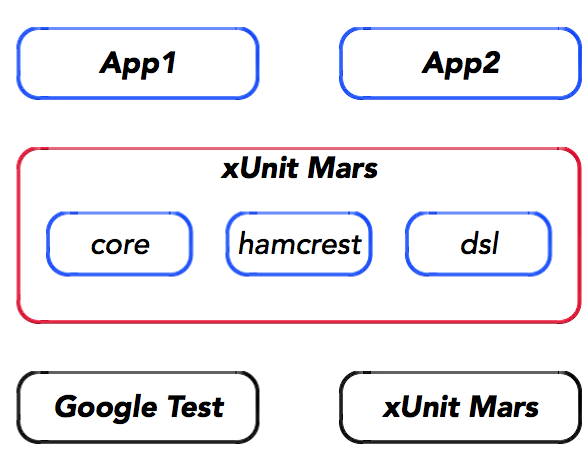
\includegraphics[width=0.5\textwidth]{figures/xunit/framework.png}
\caption{xUnit Mars: 系统架构}
 \label{fig:mars-framework}
\end{figure}

\end{content}

% \begin{savequote}[45mm]
\ascii{Any fool can write code that a computer can understand. Good programmers write code that humans can understand.}
\qauthor{\ascii{- Martin Flower}}
\end{savequote}

\chapter{破冰之旅} 
\label{ch:ice-breaker}

\begin{content}

\end{content}

\section{编程环境}

\begin{content}

\subsection{系统配置}

\begin{colortable}{X|X|X}{环境配置}
\emph{名称}                      & \emph{配置}          & \emph{版本}      \\\hline
\multirow{2}{*}\ascii{操作系统}  & \ascii{Linux Kernel} & \ascii{4.15.0}  \\\cline{2-3}
                                & \ascii{Ubuntu}       & \ascii{18.04}   \\\hline
\multirow{2}{*}\ascii{编译器}    & \ascii{GCC}          & \ascii{7.3.0}   \\\cline{2-3}
                                & \ascii{Clang}        & \ascii{6.0.0}   \\\hline
\ascii{编程语言} & \ascii{C++}   & \ascii{14}                              \\\hline
\multirow{2}{*}\ascii{构建工具}  & \ascii{CMake}        & \ascii{3.10}     \\\cline{2-3} 
                                & \ascii{Make}         & \ascii{4.10}     \\\hline
\ascii{集成开发环境}              & \ascii{Eclipse CDT}  & \ascii{Oxygen 3} \\\hline 
\ascii{版本工具}                 & \ascii{Git}          & \ascii{2.17.1}   \\\hline
\end{colortable}

\subsection{项目组织}

项目\ascii{xUnit Mars}物理目录如\refig{mars-project}所示。

\begin{figure}
\centering
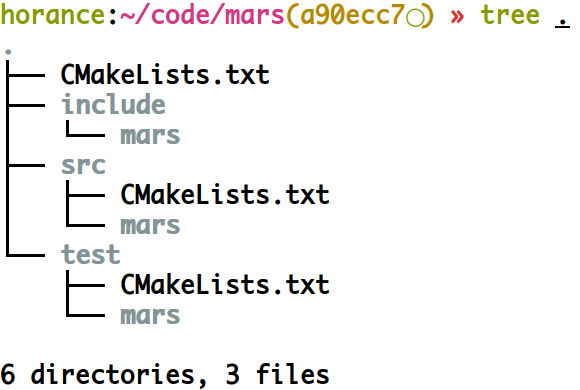
\includegraphics[width=0.6\textwidth]{figures/xunit/mars-project.png}
\caption{xUnit Mars: 项目组织}
 \label{fig:mars-project}
\end{figure}

\begin{episode}{代码风格}

\begin{content}

\emph{团队成员遵循\ascii{XP}基本价值观,致力于优秀的软件设计。}系统中所有的代码看起来就好像是由单独一个值得胜任的人编写的,并遵循一致的、统一的的代码风格。

可以配置\ascii{Eclipse CDT}代码模板,团队通过导入代码模板,使其得到一致的代码风格。业界存在多种经典的代码风格,团队应该选择并保持其中一种代码风格。

\begin{enum}
  \eitem{\code{K\&R}}
  \eitem{\code{BSD/Allman}}
  \eitem{\code{GNU}}
  \eitem{\code{Whitesmiths}}
\end{enum}

本书使用\ascii{K\&R}的代码风格,但在对齐方面做了细微调整,如\refig{eclipse-formatter}所示。配置完毕之后,便可以充分享受神奇带来的快感。

\begin{figure}[H]
\centering
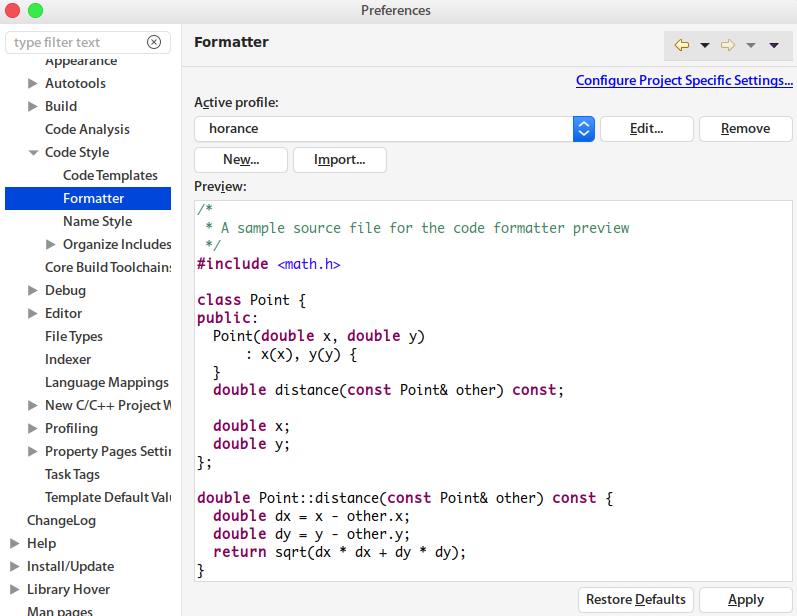
\includegraphics[width=1.0\textwidth]{figures/xunit/eclipse-formatter.png}
\caption{代码风格: K\&R}
 \label{fig:eclipse-formatter}
\end{figure}

例如,创建头文件时,自动生成\ascii{UUID}的头文件保护宏,彻底抛弃这个遗留问题;当需要排版代码时,使用快捷键\ascii{Ctrl + Shift + F}立马得到漂亮的代码风格。

关于\ascii{Eclipse CDT}详细配置与使用技巧,推荐阅读王博\footnote{\href{https://www.jianshu.com/u/92b7d9879f20}{\ascii{https://www.jianshu.com/u/92b7d9879f20}}}在简书上的三篇博文:\href{https://www.jianshu.com/p/dafcdce1f9cb}{\ascii{Effective Eclipse CDT}}。

\end{content}

\end{episode}

\subsection{构建系统}

\ascii{xUnit Mars}使用\ascii{CMake}构建工具。在项目根目录下,主控\ascii{CMakeLists.txt}完成项目的整体配置,及其子任务的组织。

\begin{nodiff}{CMakeLists.txt}
 \begin{c++}
project(mars)                                                                                  
cmake_minimum_required(VERSION 2.8)

set(CMAKE_CXX_FLAGS "${CMAKE_CXX_FLAGS} -std=c++14")

include_directories("${CMAKE_CURRENT_SOURCE_DIR}/include")

add_subdirectory(src)
add_subdirectory(test)
 \end{c++}
\end{nodiff}

\ascii{src/CMakeLists.txt}完成\ascii{mars}库构建。

\begin{nodiff}{src/CMakeLists.txt}
 \begin{c++}
file(GLOB_RECURSE all_files *.cc)
add_library(mars STATIC ${all_files})
 \end{c++}
\end{nodiff}

\ascii{test/CMakeLists.txt}完成\ascii{mars-test}应用程序构建,它执行\ascii{xUnit Mars}项目的所有测试用例。

\begin{nodiff}{test/CMakeLists.txt}
 \begin{c++}
file(GLOB_RECURSE all_files *.cc)
add_executable(mars-test ${all_files})
target_link_libraries(mars-test mars gtest gtest_main pthread)
 \end{c++}
\end{nodiff}

\subsection{Git库}

在项目根目录下初始化一个空的\ascii{Git}库。

\begin{nodiff}{初始化git库}
 \begin{c++}
$ git init
 \end{c++}
\end{nodiff}  

待项目组织完毕,完成第一次代码提交。

\begin{nodiff}{提交代码}
 \begin{c++}
$ git add -A .
$ git commit -m"setup cmake project"
 \end{c++}
\end{nodiff}

\end{content}

\section{起航}

\begin{content}

\subsection{测试用例}

万事开头难,第一个用例跑起来并不容易。此处模拟设计了一个\ascii{xUnit Mars}风格的测试用例\ascii{WasRun},它包含了一个\emph{测试方法}:\ascii{WasRun::testMethod},它是\ascii{WasRun}的一个成员函数。

\begin{nodiff}{test/mars/core/WasRunSpec.cc}
\begin{c++}
#include <gtest/gtest.h>

namespace {
  struct WasRun {
    bool wasRun = false;

    void testMethod() {
      wasRun = true;
    }
  };
}

TEST(WasRunSpec, make_sure_test_method_be_ran) {
  WasRun test;

  ASSERT_FALSE(test.wasRun);
  test.testMethod();
  ASSERT_TRUE(test.wasRun);
}
\end{c++}
\end{nodiff}

但是,这个测试很鸡肋,不仅天然地通过,而且不能驱动出任何的产品代码。再仔细思考一下,\ascii{xUnit Mars}的职责就是负责调度和执行\emph{测试方法}的,其应该对外开放执行\emph{测试方法}的\ascii{API}。因为\ascii{testMethod}是\ascii{WasRun}的一个成员函数,要调用该测试方法,必须具备两个条件:

\begin{enum}
  \eitem{测试对象:\code{WasRun}对象;}
  \eitem{测试方法:\code{WasRun::testMethod}成员函数,或指向该成员函数的指针。}
\end{enum}

因此,引入\ascii{xUnit Mars}执行测试方法的\ascii{run}函数,其第一个参数接受\ascii{WasRun}的测试对象,第二个参数接受指向成员函数\ascii{WasRun::testMethod}的指针。相比之前的测试用例,该测试可以驱动出部分实现;虽然进步甚微,但已迈出具有实际意义的第一步。

\begin{diff}{test/mars/core/WasRunSpec.cc}
\begin{minicpp}
#include <gtest/gtest.h>

namespace {
  struct WasRun {
    bool wasRun = false;

    void testMethod() {
      wasRun = true;
    }
  };
}

TEST(WasRunSpec, make_sure_test_method_be_ran) {
  WasRun test;

  ASSERT_FALSE(test.wasRun);
  test.testMethod();
  ASSERT_TRUE(test.wasRun);
}
\end{minicpp}
\tcblower
\begin{minicpp}
#include <gtest/gtest.h>

namespace {
  struct WasRun {
    bool wasRun = false;

    void testMethod() {
      wasRun = true;
    }
  };
}

TEST(WasRunSpec, make_sure_test_method_be_ran) {
  WasRun test;

  ASSERT_FALSE(test.wasRun);
  run(test, &WasRun::testMethod);
  ASSERT_TRUE(test.wasRun);
}
\end{minicpp}
\end{diff}

\begin{episode}{TDD: 测试驱动开发}

\begin{content}

\ascii{TDD}是极限编程中重要的技术实践之一。\ascii{TDD}遵循\emph{测试先行,小步快走,尽快变绿,事后重构}的基本方法论。把握\ascii{TDD}动态变化过程,做到收放自如,需要长期编程实践的经验积累。

\ascii{TDD}基本素养讲究两个字:“小”和“快”。“小”体现在测试刚好失败,实现恰如其分,重构步骤粒度甚微。而“快”体现不在于编程速度,而在于“尽最小努力,最短时间,最快通过测试”。

如果步子迈得过大,则恢复测试时间间隔会变长,信心指数则会下降,自然影响软件质量,甚至拖延软件交付进度。

\subsubsection{TDD闭环}

如\refig{tdd-cycle}所示,在一轮\ascii{TDD}编程实践过程中,遵循三部曲的闭环操作:\ascii{“Red-Green-Refactor”}。每轮迭代之后,确保系统都处于一个相对合理的状态。

\begin{figure}[H]
\centering
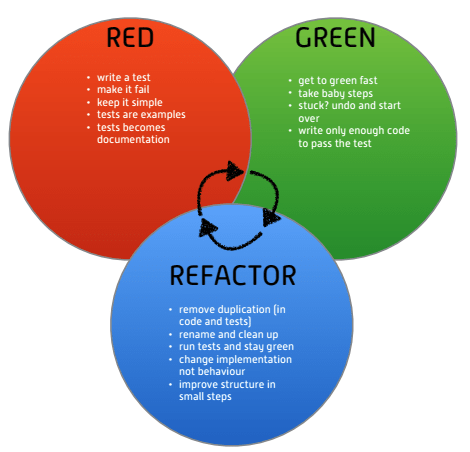
\includegraphics[width=0.8\textwidth]{figures/xunit/tdd-cycle.png}
\caption{TDD: 测试驱动开发}
 \label{fig:tdd-cycle}
\end{figure}

\subsubsection{TDD实现方法}

极限编程之父\ascii{Kent Beck}在经典著作\ascii{Test-Driven Development by Example}之中,介绍了三种基本的实现方法。

\begin{enum}
  \eitem{伪实现}
  \eitem{三角法}
  \eitem{显式实现}
\end{enum}

使用硬编码,伪装通过测试是一种最快速、最简单的实现方法。一旦通过测试,然后通过重构消除重复,以期待消除所有硬编码;或使用三角法,添加新的测试用例,驱动真实实现。

除非问题看起来并没有想象中那么简单,可以采取保守的策略也是恰当的。如果实现显而易见,完全可以绕开保守的\emph{伪实现}与\emph{三角法}。而在实际操作中,通过测试往往都比较简单,显式实现也是最常见的做法。在这种情况下,大可快速前进,不用处处敬小慎微。

\subsubsection{尽快变绿}

三种实现方法常常交替使用,虽然实现迥异,但殊途同归:以最小的努力,在最短的时间,通过测试,尽快变绿。实现过程中,尽量不要引入过度复杂的实现。例如,引入某种设计模式,重构既有的代码。

务必克服心中的恶魔,需要充分衡量成本收益比。如果引入设计较为笨重,通过测试遥遥无期,则应立即放弃;而如果引入设计显而易见,实施起来也比较容易操作,并带来一定设计的弹性,且不影响通过测试的整体进度,则可以有限接受。

\subsubsection{重构成为习惯}

一旦测试通过,务必重构既有的实现,让设计保持在目前最合理的状态。此刻,也需要克服心中的恶魔,不能做过度的设计。如果没有测试用例表达某个事件发生,则不要凭空臆想未来的世界会发生什么事情。

\subsubsection{出错后放慢脚步}

在最坏的情况下,测试在一段时间内尝试修复都以失败告终,则需要使用\ascii{Git}回退所有代码,使用更保守的\emph{伪实现}与\emph{三角法},尽快修复测试。

\subsubsection{TDD实现原则}

\ascii{Bob}大叔在其著作\ascii{Clean Code}中阐述了实践\ascii{TDD}的三个基本原则。

\begin{enum}
  \eitem{在编写不能通过的测试前,不可编写生产代码;}
  \eitem{只可编写刚好无法通过的测试,不能编译也算不通过;}
  \eitem{只可编写刚好足以通过当前失败测试的生产代码。}
\end{enum}

理解起来比较绕口,换一个等价的、较易理解的方式,可以表述为:

\begin{enum}
  \eitem{测试先行;}
  \eitem{测试失败;}
  \eitem{尽快变绿。}
\end{enum}

\subsubsection{TDD实现技巧}

实践\ascii{TDD}时,常需要规划和维护一个\ascii{TODO List}。将熟悉的,价值大,容易实现,高优先级的测试用例优先实现;而将不熟悉,价值小,不易实现,异常边界的测试用例依次排到后面,留待后续处理。

\begin{enum}
  \eitem{基本功能与异常场景;}  
  \eitem{高价值与现成果实;}
  \eitem{确定与不确定;}
  \eitem{整体优先与细节优先。}
\end{enum}

\end{content}

\end{episode}

\subsubsection{通过测试}

不幸的是,\ascii{run}函数依赖于具体类型\ascii{WasRun},而\ascii{WarRun}存在于匿名命名空间内。我们不期望将\ascii{WasRun}搬迁至产品实现中,毕竟\ascii{WarRun}是一个用户自定义的\ascii{xUnit Mars}风格的测试用例。

为了快速通过测试用例,且不破坏匿名命名空间的封装性,姑且就近实现\ascii{run}函数,暂时不搬迁\ascii{run}函数至产品代码之中。

\begin{nodiff}{test/mars/core/WasRunSpec.cc}
\begin{c++}
#include <gtest/gtest.h>

namespace {
  struct WasRun {
    bool wasRun = false;

    void testMethod() {
      wasRun = true;
    }
  };

  void run(WasRun& self, void(WasRun::*method)()) {
    (self.*method)();
  }
}

TEST(WasRunSpec, make_sure_test_method_be_ran) {
  WasRun test;
  ASSERT_FALSE(test.wasRun);

  run(test, &WasRun::testMethod);
  ASSERT_TRUE(test.wasRun);
}
\end{c++}
\end{nodiff}

\subsubsection{执行测试}

在\ascii{build}临时目录中,使用\ascii{cmake}构建工程。

\begin{nodiff}{构建工程}
 \begin{c++}
$ mkdir -p build && cd build
$ cmake ..
$ make
 \end{c++}
\end{nodiff}

运行测试。

\begin{nodiff}{运行测试}
 \begin{c++}
$ test/mars-test
Running main() from gtest_main.cc
[==========] Running 1 test from 1 test case.
[----------] Global test environment set-up.
[----------] 1 test from SimpleTest
[ RUN      ] SimpleTest.make_sure_test_case_can_run_normally
[       OK ] SimpleTest.make_sure_test_case_can_run_normally (0 ms)
[----------] 1 test from SimpleTest (0 ms total)

[----------] Global test environment tear-down
[==========] 1 test from 1 test case ran. (0 ms total)
[  PASSED  ] 1 test.
 \end{c++}
\end{nodiff}

\begin{episode}{全局忽略模式}

\begin{content}

\ascii{CMake}在临时目录\ascii{build}中完成系统构建,为了避免不经意地将\ascii{build}目录提交至\ascii{Git}库,常常需要在\ascii{.gitignore}文件中配置相应的忽略模式。

但是,为每个项目都创建一个\ascii{.gitignore}文件,显然是一种重复设计。因此,配置全局忽略模式是一个更恰当的解决方案。

 \begin{c++}
$ git config --global core.excludesfile ~/.gitignore_global
$ vi ~/.gitignore_global
# cmake
build/

# vi
*.swp

# eclipse
.project
.cproject
.settings/

# tex
output/
 \end{c++}

\end{content}
\end{episode}

\subsubsection{提交代码}

每当通过测试后,立即提交代码到\ascii{Git}库。

\begin{nodiff}{提交代码}
 \begin{c++}
$ git add -A .
$ git commit -m"pass first test case"
 \end{c++}
\end{nodiff}

\begin{episode}{后悔药}

\begin{content}

感谢\ascii{Linus}创造了\ascii{Linux}与\ascii{Git},让全世界的程序员得以享受编程的快乐。\ascii{TDD}精髓之一便是“小”,配合运用\ascii{Git},简直就是完美,避免不经意的错误而丢失代码。

养成经常性提交代码至\ascii{Git}库,是一种良好的编程习惯。在\ascii{TDD}的一个迭代循环中,每当编译通过,链接通过,测试通过,关键重构成功,都应立即执行\ascii{git add}。当设计重构至相对合理状态,最后执行\ascii{git commit}入库,完成一次\ascii{TDD}的闭环。

此外,借助于\ascii{Git},随时可以吃后悔药。当尝试某种重构设计时,没有达到预期效果,则可以轻松回到上一个稳定状态,重新开始尝试新的努力。以“重命名函数”的重构过程为例,讲述\ascii{Git}的操作。

\begin{enum}
  \eitem{新建一个函数;}
  \eitem{拷贝旧函数的实现至新函数;}
  \eitem{确保编译、测试通过,执行\code{git add};}  
  \eitem{删除旧函数的实现逻辑,转调新函数;}
  \eitem{确保编译、测试通过,执行\code{git add};}
  \eitem{对于每个引用旧函数的地方,重构引用新函数,确保编译、测试通过,执行\code{git add};}    
  \eitem{删除旧函数,确保编译、测试通过,执行\code{git commit}。}      
\end{enum}

\end{content}
\end{episode}

\subsection{引入泛型}

设计的坏味道非常明显,\ascii{run}函数与\ascii{WasRun}类型强度耦合,不够泛化。不仅无法搬迁\ascii{run}函数到产品代码中,而且不易被其他测试用例复用。例如,增加测试用例\ascii{WasSucc},不得不再重复实现\ascii{run}函数的逻辑。

\begin{diff}{test/mars/core/WasRunSpec.cc, test/mars/core/WasSuccSpec.cc}
\begin{minicpp}
#include <gtest/gtest.h>

namespace {
  struct WasRun {
    bool wasRun = false;

    void testMethod() {
      wasRun = true;
    }
  };

  void run(WasRun& self, void(WasRun::*method)()) {
    (self.*method)();
  }
}

TEST(WasRunSpec, make_sure_test_method_be_ran) {
  WasRun test;

  ASSERT_FALSE(test.wasRun);
  run(test, &WasRun::testMethod);
  ASSERT_TRUE(test.wasRun);
}
\end{minicpp}
\tcblower
\begin{minicpp}
#include <gtest/gtest.h>

namespace {
  struct WasSucc {
    bool wasSucc = false;

    void testMethod() {
      wasSucc = true;
    }
  };

  void run(WasSucc& self, void(WasSucc::*method)()) {
    (self.*method)();
  }
}

TEST(WasRunSpec, make_sure_test_method_be_ran) {
  WasSucc test;

  ASSERT_FALSE(test.wasSucc);
  run(test, &WasSucc::testMethod);
  ASSERT_TRUE(test.wasSucc);
}
\end{minicpp}
\end{diff}

虽然两个测试用例是通过的,但两个特化实现的\ascii{run}函数引入了重复设计。为了消除两者实现的重复设计,可以引入泛型设计。此时,可以在产品代码中创建泛型函数\ascii{run},并简单实现以消除两个特化实现的\ascii{run}函数。

\begin{nodiff}{include/mars/core/TestMethod.h}
\begin{c++}
#ifndef HD3E38C9A_3B03_48CE_9A1B_75B41CB012C6
#define HD3E38C9A_3B03_48CE_9A1B_75B41CB012C6

template <typename Fixture>
void run(Fixture& self, void(Fixture::*method)()) {
  (self.*method)();
}

#endif
\end{c++}
\end{nodiff}

\begin{episode}{头文件保护宏}

\begin{content}

\ascii{C/C++}编译模型通过使用\ascii{include}语句导入头文件而实现的。为了避免头文件被导入多次,每一个头文件都应该定义独一无二的头文件保护宏。社区存在两种典型的代码风格:

\begin{enum}
  \eitem{\code{INCL\_<PROJECT>\_<MODULE>\_<FILE>\_H}}
  \eitem{\code{UUID}}
\end{enum}

第一种命名风格问题在于:当头文件被重命名或移动目录时,为了保持一致性需要同步修改头文件保护宏,而此特性\ascii{IDE}通常支持都不是太良好。因此,推荐随机生成\ascii{UUID},其更加快捷、简单、并且安全、有效。

首先,配置\ascii{Eclipse CDT}的代码模板。当创建头文件时,自动生成头文件保护宏。

\begin{figure}[H]
\centering
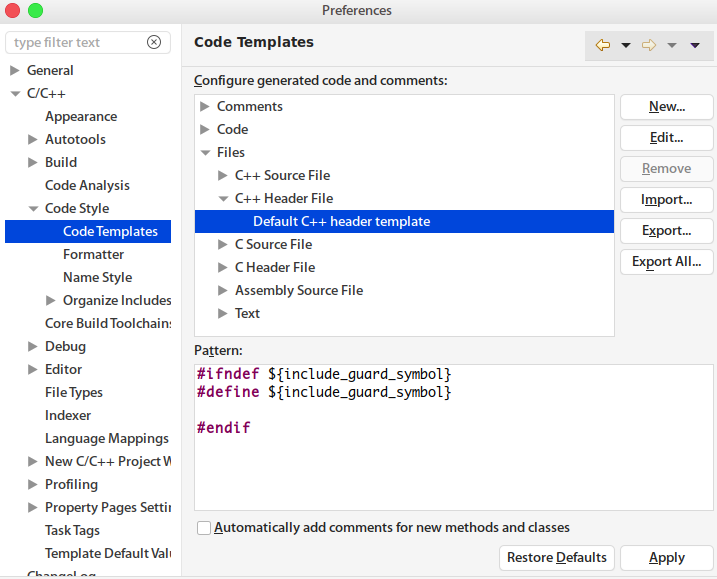
\includegraphics[width=0.95\textwidth]{figures/xunit/eclipse-code-template.png}
\caption{Eclipse CDT: 代码模板}
 \label{fig:eclipse-code-template}
\end{figure}

然后,配置头文件保护宏使用\ascii{UUID}自动生成。

\begin{figure}[H]
\centering
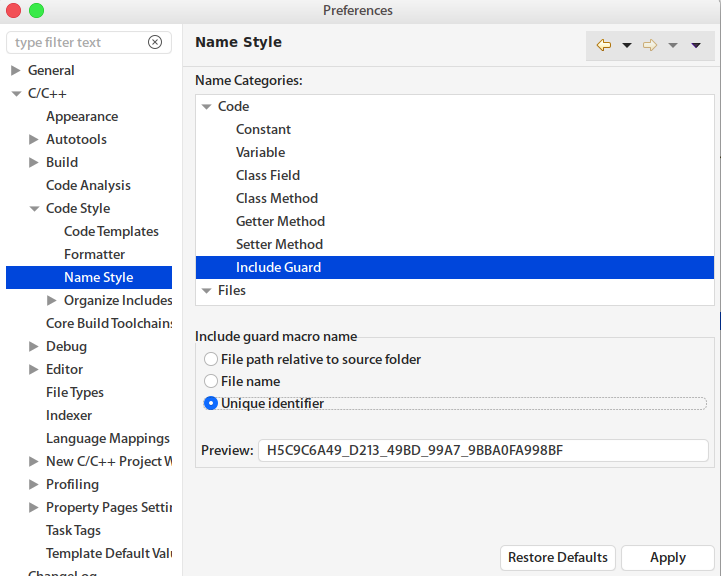
\includegraphics[width=0.95\textwidth]{figures/xunit/eclipse-include-guard.png}
\caption{Eclipse CDT: 生成UUID的头文件保护宏}
 \label{fig:eclipse-include-guard}
\end{figure}

为了缩短篇幅,后文略去所有头文件保护符。

\end{content}
\end{episode}

以\ascii{WasRunSpec.cc}为例,使用泛化的\ascii{run}函数,替代特化的\ascii{run}函数,其效果如下所示。同理,\ascii{WasSuccSpec.cc}使用相同的重构方法应用泛化的\ascii{run}函数。最终消除了两者之间的重复设计,并驱动出产品的初始代码。

\begin{nodiff}{test/mars/core/WasRunSpec.cc}
\begin{c++}
#include <mars/core/TestMethod.h>
#include <gtest/gtest.h>

namespace {
  struct WasRun {
    bool wasRun = false;

    void testMethod() {
      wasRun = true;
    }
  };
}

TEST(WasRunSpec, make_sure_test_method_be_ran) {
  WasRun test;

  ASSERT_FALSE(test.wasRun);
  run(test, &WasRun::testMethod);
  ASSERT_TRUE(test.wasRun);
}
\end{c++}
\end{nodiff}

\subsection{自动实例}

\ascii{run}函数虽然已经泛化了,但是它仅仅实现了测试方法的间接调用,其职责也很鸡肋。再次深入客户场景分析,用户更期待能够直接执行\emph{测试方法},并不期望\emph{测试对象}的创建和维护。重构既有测试用例使其失败,使其\ascii{run}函数不再依赖于具体的测试对象。

\begin{diff}{test/mars/core/WasSuccSpec.cc}
\begin{minicpp}
#include <mars/core/TestMethod.h>
#include <gtest/gtest.h>

namespace {
  struct WasRun {
    bool wasRun = false;

    void testMethod() {
      wasRun = true;
    }
  };
}

TEST(WasRunSpec, make_sure_test_method_be_ran) {
  WasRun test;

  ASSERT_FALSE(test.wasRun);
  run(test, &WasRun::testMethod);
  ASSERT_TRUE(test.wasRun);
}
\end{minicpp}
\tcblower
\begin{minicpp}
#include <mars/core/TestMethod.h>
#include <gtest/gtest.h>

namespace {
  bool wasRun = false;

  struct WasRun {
    void testMethod() {
      wasRun = true;
    }
  };
}

TEST(WasRunSpec, make_sure_test_method_be_ran) {
  ASSERT_FALSE(wasRun);
  run(&WasRun::testMethod);
  ASSERT_TRUE(wasRun);
}
\end{minicpp}
\end{diff}

为了能够快速通过测试,泛化的\ascii{run}函数额外承担测试对象创建和维护的职责。

\begin{diff}{include/mars/core/TestMethod.h}
\begin{minicpp}
template <typename Fixture>
void run(Fixture& self, void(Fixture::*method)()) {
  (self.*method)();
}
\end{minicpp}
\tcblower
\begin{minicpp}
template <typename Fixture>
void run(void(Fixture::*method)()) {
  Fixture self;
  (self.*method)();
}
\end{minicpp}
\end{diff}

\subsection{函数对象}

泛型的\ascii{run}函数,使其持有和维护\emph{测试对象},限制了\emph{测试对象}的生命周期。引入\emph{函数对象},替代\ascii{run}函数。重构既有的测试用例,使用函数对象\ascii{TestMethod}替代泛型函数\ascii{run}。

\begin{diff}{test/mars/core/WasRunSpec.cc}
\begin{minicpp}
#include <mars/core/TestMethod.h>
#include <gtest/gtest.h>

namespace {
  bool wasRun = false;

  struct WasRun {
    void testMethod() {
      wasRun = true;
    }
  };
}

TEST(WasRunSpec, make_sure_test_method_was_ran) {
  ASSERT_FALSE(wasRun);
  run(&WasRun::testMethod);
  ASSERT_TRUE(wasRun);
}
\end{minicpp}
\tcblower
\begin{minicpp}
#include <mars/core/TestMethod.h>
#include <gtest/gtest.h>

namespace {
  bool wasRun = false;

  struct WasRun {
    void testMethod() {
      wasRun = true;
    }
  };
}

TEST(WasRunSpec, make_sure_test_method_was_ran) {
  TestMethod<WasRun> test(&WasRun::testMethod);

  ASSERT_FALSE(wasRun);
  test.run();
  ASSERT_TRUE(wasRun);
}
\end{minicpp}
\end{diff}

为了通过测试,引入函数对象\ascii{TestMethod},它搬迁泛型函数\ascii{run}的主干逻辑。

\begin{diff}{include/mars/core/TestMethod.h}
\begin{minicpp}
template <typename Fixture>
void run(void(Fixture::*method)()) {
  Fixture self;
  (self.*method)();
}
\end{minicpp}
\tcblower
\begin{minicpp}
template <typename Fixture>
struct TestMethod {
private:
  using Method = void(Fixture::*)();

public:
  TestMethod(Method method)
    : method(method) {
  }

  void run() {
    (self.*method)();
  }

private:
  Fixture self;
  Method method;
};
\end{minicpp}
\end{diff}

此时,\ascii{TestMethod}持有\emph{测试对象},并负责执行\emph{测试方法}。相对于普通函数,\ascii{TestMethod}更加具有设计弹性,可以维持其状态实施存储操作。


需要关注的是,\ascii{TestCase}实现了一个虚拟析构函数。如果不经意地遗忘声明该析构函数为虚拟的\footnote{默认生成的析构函数是公开的、非虚拟的、内联实现的。},则可能招致运行时不确定的行为发生。

\begin{episode}{虚拟析构函数}
\begin{content}

一般地,需要为\emph{多态基类}声明虚拟析构函数;否则,会招致运行时不可预期的行为。一般地,如果一个类包含虚函数时,便将其析构函数声明为虚拟的。

\subsubsection{空实现}

但是,为每个接口类型实现一个空的虚拟析构函数,显得重复而且麻烦。可以引入一个宏定义,自动引入空实现的虚拟析构函数。

 \begin{c++}
namespace details {
  template<typename T>
  struct Trait {
    virtual ~Trait() {}
  };
}

#define TRAIT(trait)  struct trait : ::details::Trait<trait>
#define EXTENDS(...) , ##__VA_ARGS__
 \end{c++}

例如,使用\ascii{TRAIT}宏,定义了一个接口类型\ascii{SelfDescribing},它自动拥有虚拟析构函数的默认空实现。

 \begin{c++}
struct Description;

TRAIT(SelfDescribing) {
  virtual void describeTo(Description& desc) const = 0;
};
 \end{c++}

\subsubsection{抽象函数}

此外,定义纯虚函数时,常常会遗忘后面的\ascii{0}。可以引入另外一个宏定义。

 \begin{c++}
#define ABSTRACT(...) virtual __VA_ARGS__ = 0
 \end{c++}

使用\ascii{ABSTRACT}定义,不仅可以抑制不经意地遗漏\ascii{0}的错误,也可以改善\ascii{API}的意图和可读性。

\begin{c++}
struct Description;

TRAIT(SelfDescribing) {
  ABSTRACT(void describeTo(Description& desc) const);
};
\end{c++}

\end{content}
\end{episode}

\subsection{通过链接}

创建一个空的\ascii{TestCase.cc}文件,这里仅为了\ascii{libmars.a}不为空,保证\ascii{CMake}构建系统工作正常;否则,\ascii{CMake}提示\ascii{mars}项目为空,无法构建\ascii{libmars.a}库。

\begin{nodiff}{src/mars/core/TestCase.cc}
 \begin{c++}
#include "mars/core/TestCase.h"
 \end{c++}
\end{nodiff}

\begin{episode}{多屏编辑}

\begin{content}

在\cpp{}编程实践中,需要在头文件和实现文件之间频繁切换。同时,在\ascii{TDD}编程实践中,也需要在测试文件与头文件/实现文件之间频繁切换。

得益于现代\ascii{IDE}的丰富特性,推荐多屏显示相关源文件。例如,如\refig{multi-editor-eclipse}所示,使用\ascii{Eclipse CDT},三屏分别显示相关联的头文件、实现文件,及其测试用例文件。

\begin{figure}[H]
\centering
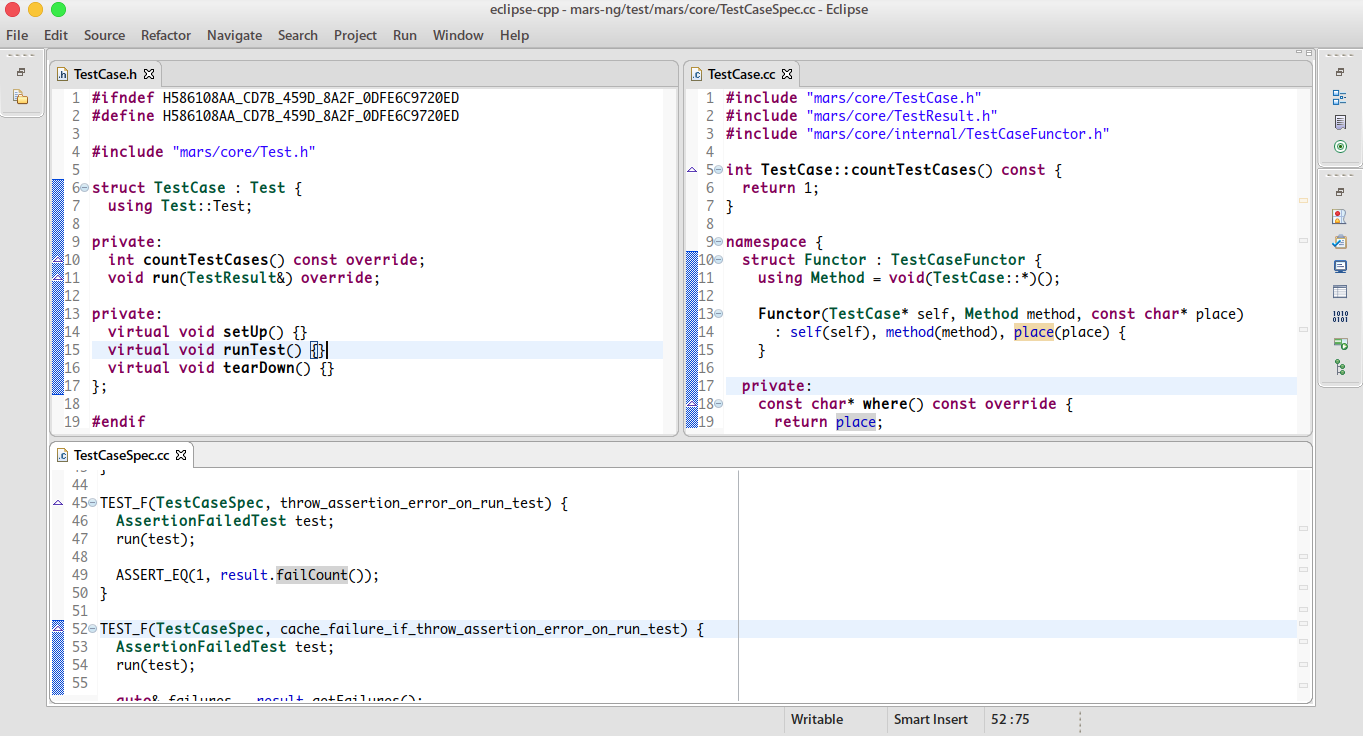
\includegraphics[width=1.0\textwidth]{figures/xunit/multi-editor-eclipse.png}
\caption{Eclipse CDT: 多屏显示}
 \label{fig:multi-editor-eclipse}
\end{figure}

推荐购置高清,大屏显示器,有效改善编程环境,从而提高工作效率。关闭无关的\ascii{Tab}页,只打开当前相关的文件,最小化外部干扰;一则让\ascii{IDE}运行速度最佳,二则使用诸如\ascii{Ctrl + E}快捷键切换文件时,最小化文件列表长度。

强烈推荐使用快捷键的优秀实践,可以成倍地提高编程的效率。例如,使用快捷键\ascii{Ctrl + Tab},在头文件与实现文件间切换自如。

\end{content}

\end{episode}

\end{content}


% \begin{savequote}[45mm]
\ascii{Any fool can write code that a computer can understand. Good programmers write code that humans can understand.}
\qauthor{\ascii{- Martin Flower}}
\end{savequote}

\chapter{算法骨架} 
\label{ch:skeleton}

\begin{content}

\end{content}

\section{前置}

\begin{content}

一般地,在执行测试前需要预置\ascii{setUp}实施测试环境的初始化工作,完成资源的准备。对既有的用例实施重构。

\subsection{测试用例}

\begin{leftbar}
 \begin{c++}[caption={\ttfamily{test/mars/core/TestCaseSpec.cc}}]
#include <gtest/gtest.h>
#include "mars/core/TestCase.h"

namespace {
  struct SimpleTest : TestCase {
    bool wasSetUp = false;
    bool wasRun = false;

  private:
    void setUp() override {
      wasSetUp = true;
    }

    void runTest() override {
      wasRun = true;
    }
  };
}

TEST(SimpleTest, make_sure_test_case_can_run_normally) {
  SimpleTest test;
  test.run();

  ASSERT_TRUE(test.wasSetUp);
  ASSERT_TRUE(test.wasRun);
}
 \end{c++}
\end{leftbar}

\begin{story}
  \begin{center}
    \inlinetitle{private与override}
  \end{center}

\begin{content}

感谢\ascii{Linus}创造了\ascii{Linux}与\ascii{Git},让全世界的程序员得以享受编程的快乐。\ascii{TDD}精髓之一便是“小”,配合运用\ascii{Git},简直就是完美,避免不经意的错误而丢失代码。

养成经常性提交代码至\ascii{Git}库,是一种良好的编程习惯。在\ascii{TDD}的一个迭代循环中,每当编译通过,链接通过,测试通过,完成重构等关键环节,都立即执行\ascii{git add}。当设计重构至相对合理状态,执行\ascii{git commit}入库。在任何时刻,都可回溯至上一个稳定的状态。如\refig{tdd-git}所示。

借助于\ascii{Git},随时可以吃后悔药。当尝试某种重构设计时,没有达到预期效果,则可以轻松回到上一个稳定状态,开始尝试新的努力。

\begin{figure}[H]
\centering
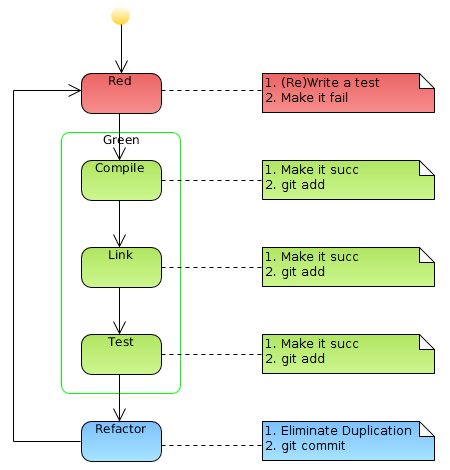
\includegraphics[width=0.6\textwidth]{figures/xunit/tdd-git.png}
\caption{TDD环: 关键环节提交代码}
 \label{fig:tdd-git}
\end{figure}

\end{content}

\end{story}

\subsection{通过编译}

重构\ascii{TestCase},仅公开\ascii{run}方法,并移除运行时多态的特性,它负责组织用例执行运行时的算法骨架。搬迁运行时多态行为至私有的两个虚函数,用户根据自己的场景定制\ascii{setUp}与\ascii{runTest},分别完成测试准备,及其测试执行。

\begin{leftbar}
 \begin{c++}[caption={\ttfamily{include/mars/core/TestCase.h}}]
struct TestCase {
  virtual ~TestCase() {}

  void run();

private:
  virtual void setUp() {}
  virtual void runTest() {}
};
  \end{c++}
\end{leftbar}

\subsection{通过测试}

实现\ascii{TestCase::run}的主体逻辑。

\begin{leftbar}
 \begin{c++}[caption={\ttfamily{src/mars/core/TestCase.cc}}]
#include "mars/core/TestCase.h"

void TestCase::run() {
  setUp();
  runTest();
}
 \end{c++}
\end{leftbar}

测试通过。

\end{content}

\section{后置}

\begin{content}

\subsection{测试用例}

同理,测试执行后使用\ascii{tearDown}完成现场清理,释放资源。用户通过定制私有的虚函数\ascii{tearDown}完成此功能。

\begin{leftbar}
 \begin{c++}[caption={\ttfamily{test/mars/core/TestCaseSpec.cc}}]
#include <gtest/gtest.h>
#include "mars/core/TestCase.h"

namespace {
  struct SimpleTest : TestCase {
    bool wasSetUp = false;
    bool wasRun = false;
    bool wasTearDown = false;

  private:
    void setUp() override {
      wasSetUp = true;
    }

    void runTest() override {
      wasRun = true;
    }

    void tearDown() override {
      wasTearDown = true;
    }
  };
}

TEST(SimpleTest, make_sure_test_case_can_run_normally) {
  SimpleTest test;
  test.run();

  ASSERT_TRUE(test.wasSetUp);
  ASSERT_TRUE(test.wasRun);
  ASSERT_TRUE(test.wasTearDown);  
}
 \end{c++}
\end{leftbar}

\subsection{通过编译}

当用例执行完成后,\ascii{TestCase::tearDown}负责清理现场。

\begin{leftbar}
 \begin{c++}[caption={\ttfamily{include/mars/core/TestCase.h}}]
struct TestCase {
  virtual ~TestCase() {}

  void run();

private:
  virtual void setUp() {}
  virtual void runTest() {}
  virtual void tearDown() {}
};
  \end{c++}
\end{leftbar}

\subsection{通过测试}

至此,完成了运行一个用例的主干逻辑,但缺乏异常处理机制,留待后续处理。

\begin{leftbar}
 \begin{c++}[caption={\ttfamily{src/mars/core/TestCase.cc}}]
#include "mars/core/TestCase.h"

void TestCase::run() {
  setUp();
  runTest();
  tearDown();
}
 \end{c++}
\end{leftbar}

\end{content}

\section{算法骨架}

\begin{content}

\ascii{TestCase::run}实现了\ascii{xUnit}最核心的高层算法逻辑,实现了高层算法逻辑与底层实现细节的解耦,并且实现了高层算法逻辑的高度复用。如\refig{simple-test}所示。

\begin{figure}[H]
\centering
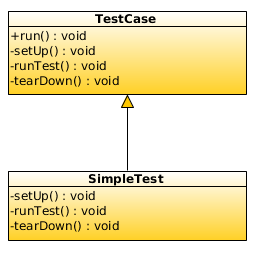
\includegraphics[width=0.4\textwidth]{figures/xunit/simple-test.png}
\caption{模板方法:定义算法骨架}
 \label{fig:simple-test}
\end{figure}

\subsection{引入策略}

模板方法模式与策略模式都可以用来分离高层的算法与具体的实现细节。之前已经看到了模板方法的实现,接下来探讨策略模式实现的效果,并从中对比两者之间的差异,从而指导设计的权衡与取舍。

\subsubsection{测试用例}

\ascii{TestCaseRunner}构建高层算法逻辑,而\ascii{TestCase}作为\ascii{TestCaseRunner}的抽象策略。新增测试用时,覆写\ascii{TestCase}相关接口,完成具体实现细节。实现\ascii{TestCaseRunner}的高层算法逻辑与\ascii{SimpleTest}的具体实现细节之间关系的解耦。

\begin{leftbar}
 \begin{c++}
namespace {
  struct SimpleTest : TestCase {
    bool wasSetUp = false;
    bool wasRun = false;
    bool wasTearDown = false;

  private:
    void setUp() override {
      wasSetUp = true;
    }

    void runTest() override {
      wasRun = true;
    }

    void tearDown() override {
      wasTearDown = true;
    }
  };
}

TEST(SimpleTest, run_test_case_using_strategry) {
  SimpleTest test;
  TestRunner runner(test);
  runner.run();

  ASSERT_TRUE(test.wasSetUp);
  ASSERT_TRUE(test.wasRun);
  ASSERT_TRUE(test.wasTearDown);  
}
 \end{c++}
\end{leftbar}

\subsubsection{通过测试}

\ascii{TestRunner::run}负责组织高层算法逻辑,算法子步骤的实现通过抽象的\ascii{TestCase}委托给某个具体策略对象完成。从而实现了\ascii{TestCaseRunner}与\ascii{SimpleTest}之间的解耦,两者都依赖于抽象的\ascii{TestCase},如\refig{simple-test-strategry}所示。

\begin{figure}[H]
\centering
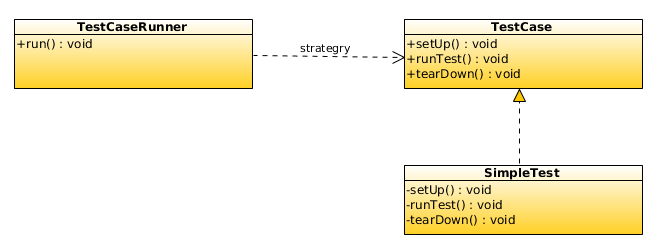
\includegraphics[width=1.0\textwidth]{figures/xunit/simple-test-strategry.png}
\caption{策略对象:定义算法骨架}
 \label{fig:simple-test-strategry}
\end{figure}


\begin{leftbar}
 \begin{c++}
struct TestCase {
  virtual ~TestCase() {}

  virtual void setUp() {}
  virtual void runTest() {}
  virtual void tearDown() {}
};

struct TestCaseRunner {
  TestCaseRunner(TestCase& test) : test(test) {
  }

  void run() {
    test.setUp();
    test.runTest();
    test.tearDown();
  }

private:
  TestCase& test;
};
 \end{c++}
\end{leftbar}

\subsection{权衡利弊}

使用模板方法,\ascii{SimpleTest}通过继承方式直接复用了\ascii{TestCase::run}高层算法逻辑。但继承是一种强依赖,增强了\ascii{SimpleTest}与\ascii{TestCase}之间的耦合关系。

使用策略方法,\ascii{TestCaseRunner}高层算法逻辑与\ascii{SimpleTest}是解耦的,但额外地引入类\ascii{TestCaseRunner}。

既然两个方案都有优缺点,到底应该采用哪个方案呢?其一,使用策略方法,需要建立额外的委托关系,不仅增加过多的类,使得设计变得更加复杂。其二,观察\ascii{TestCaseRunner::run}的实现,其实现基本完全委托给了\ascii{TestCase};按照迪米特法则,这段高层算法逻辑应该归属于\ascii{TeseCase}。

\begin{leftbar}
\begin{c++}
void TestCaseRunner::run() {
  test.setUp();
  test.runTest();
  test.tearDown();
}
\end{c++}
\end{leftbar}

按照这个推理,实施重构将\ascii{TestCaseRunner::run}搬迁至\ascii{TestCase},\ascii{TestCaseRunner}就成为一个空类,根本就没有存在的理由。因此,按照迪米特法则,也应优选模板方法。

如果优选模板方法,那么需要分析一下此场景使用模板方法的带来的副作用。无非就是因为引入继承关系从而增强了\ascii{TestCase}与\ascii{SimpleTest}的耦合关系。但是,考虑到\ascii{SimpleTest}是\ascii{xUnit Mars}最小调度单位,不会进一步被继承或组合而被复用,这个耦合关系仅局部于\ascii{SimpleTest}内部,不会被传播到其他地方,这是完全可以接受的设计。



\end{content}

% \begin{savequote}[45mm]
\ascii{Any fool can write code that a computer can understand. Good programmers write code that humans can understand.}
\qauthor{\ascii{- Martin Flower}}
\end{savequote}

\chapter{隐式树} 
\label{ch:implicit-tree}

\begin{content}

\end{content}

\section{测试套件}

\begin{content}

如果每个用例都需要手动地执行\ascii{run},显得极其笨拙。可以将一堆测试用例打包,用一个简单的\ascii{for}循环依次执行每个用例。

\subsection{测试用例}

为了确定每个\ascii{TestCase}都被执行,可以简单定制一个计数器\ascii{num},用例执行后,断言已运行用例的数目。

\begin{leftbar}
 \begin{c++}[caption={\ttfamily{test/mars/core/TestSuiteSpec.cc}}]
#include <gtest/gtest.h>
#include "mars/core/TestCase.h"
#include "mars/core/TestSuite.h"

namespace {
  int num = 0;

  struct FooTest : TestCase {
  private:
    void runTest() override {
      num++;
    }
  };
}

TEST(TestSuite, run_multi_test_cases_using_test_suite) {
  TestSuite suite;
  suite.add(new FooTest);
  suite.add(new FooTest);

  suite.run();

  ASSERT_EQ(2, num);
}
 \end{c++}
\end{leftbar}

\subsection{通过编译}

为了快速通过编译,创建\ascii{TestSuite}的头文件。

\begin{leftbar}
 \begin{c++}[caption={\ttfamily{include/mars/core/TestSuite.h}}]
#include <vector>

struct TestCase;

struct TestSuite {
  void add(TestCase* test);
  void run();

private:
  std::vector<TestCase*> tests;
};
 \end{c++}
\end{leftbar}

\subsection{通过测试}

为了通过测试,可以快速实现\ascii{TestSuite::run}的逻辑。

\begin{leftbar}
 \begin{c++}[caption={\ttfamily{src/mars/core/TestSuite.cc}}]
#include "mars/core/TestSuite.h"
#include "mars/core/TestCase.h"

void TestSuite::add(TestCase* test) {
  tests.push_back(test);
}

void TestSuite::run() {
  for (auto test : tests) {
    test->run();
  }
}
 \end{c++}
\end{leftbar}

\subsection{内存泄露}

\ascii{TestSuite}持有若干\ascii{TestCase}实例,引入析构函数释放动态创建并添加至\ascii{TestSuite}的所有\ascii{TestCase}实例。

\begin{leftbar}
 \begin{c++}[caption={\ttfamily{include/mars/core/TestSuite.h}}]
#include <vector>

struct TestCase;

struct TestSuite {
  ~TestSuite();

  void add(TestCase* test);
  void run();

private:
  std::vector<TestCase*> tests;
};
 \end{c++}
\end{leftbar}

实现析构函数,释放动态内存。

\begin{leftbar}
 \begin{c++}[caption={\ttfamily{src/mars/core/TestSuite.cc}}]
#include "mars/core/TestSuite.h"
#include "mars/core/TestCase.h"

void TestSuite::add(TestCase* test) {
  tests.push_back(test);
}

TestSuite::~TestSuite() {
  for (auto test : tests) {
    delete test;
  }
}

void TestSuite::run() {
  for (auto test : tests) {
    test->run();
  }
}
 \end{c++}
\end{leftbar}

\subsection{消除重复}

为了消除析构函数与\ascii{run}之间的重复代码,提取一个公共的\ascii{foreach}函数。注意,不要在头文件直接实现该模板函数,最小化编译时的依赖。

\begin{leftbar}
 \begin{c++}[caption={\ttfamily{include/mars/core/TestSuite.h}}]
#include <vector>

struct TestCase;

struct TestSuite {
  ~TestSuite();

  void add(TestCase* test);
  void run();

private:
  template <typename F>
  void foreach(F f) const;

private:
  std::vector<TestCase*> tests;
};
 \end{c++}
\end{leftbar}

因此,设计得到两个独立变化的方向。

\begin{enum}
  \eitem{\ascii{迭代算法:因存储结构变化而变化(目前实现为线性列表,不排除将来实现为map);}}
  \eitem{\ascii{处理算子:存在删除,计数,运行等操作。}}
\end{enum}

可以使用\ascii{Lambda}表达式定制各种算子,实现差异化配置,实现对迭代算法的高度复用。

\begin{leftbar}
 \begin{c++}[caption={\ttfamily{src/mars/core/TestSuite.cc}}]
#include "mars/core/TestSuite.h"
#include "mars/core/TestCase.h"

void TestSuite::add(TestCase* test) {
  tests.push_back(test);
}

template <typename F>
inline void TestSuite::foreach(F f) const {
  for (auto test : tests) {
    f(test);
  }
}

TestSuite::~TestSuite() {
  foreach([](auto test) {
    delete test;
  });
}

void TestSuite::run() {
  foreach([](auto test) {
    test->run();
  });
}
 \end{c++}
\end{leftbar}

\section{嵌套结构}

为了实现更好的可扩展性,\ascii{TestSuite}不仅能打包\ascii{TestCase}实例,也应该能够打包更小的\ascii{TestSuite}的子实例,实现隐式的树结构。


\begin{figure}[H]
\centering
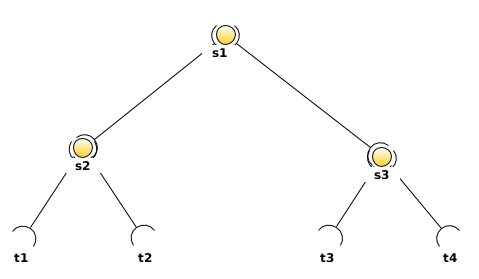
\includegraphics[width=0.8\textwidth]{figures/xunit/test-tree-example.png}
\caption{用例树:TestSuite(s1, s2, s3),TestCase(t1,t2,t3,t4)}
 \label{fig:test-case-tree}
\end{figure}

\subsection{测试依赖}

为了能够添加更多的用例,需要对计数器\ascii{num}实施初始化。当执行用例时,确保\ascii{num}被初始化为\ascii{0};否则测试用例之间存在数据脏写的错误依赖。另外,此处没有直接调用\ascii{TestSuite::run},而是使用更为抽象的\ascii{Test::run},测试装置将更加稳定。

在实现\ascii{TestSuiteSpec::run}时,显式地使用域限定符\ascii{::Test},避免与\ascii{testing::Test}产生二义性而导致编译失败。

\begin{leftbar}
 \begin{c++}[caption={\ttfamily{test/mars/core/TestSuiteSpec.cc}}]
#include <gtest/gtest.h>
#include "mars/core/TestCase.h"
#include "mars/core/TestSuite.h"

namespace {
  int num = 0;

  struct FooTest : TestCase {
  private:
    void runTest() override {
      num++;
    }
  };

  struct TestSuiteSpec : testing::Test {
  private:
    void SetUp() override {
      num = 0;  // IMPORTANT: reset counter.
    }

  protected:
    void run(::Test& test) {
      test.run();
    }
  };
}

TEST_F(TestSuiteSpec, package_multi_test_cases_into_test_suite) {
  TestSuite suite;
  suite.add(new FooTest);
  suite.add(new FooTest);

  run(suite);

  ASSERT_EQ(2, num);
}

TEST_F(TestSuiteSpec, package_sub_test_suite_into_outter_test_suite) {
  auto inner = new TestSuite;
  inner->add(new FooTest);

  TestSuite outter;
  outter.add(new FooTest);
  outter.add(inner);

  run(outter);

  ASSERT_EQ(2, num);
}
 \end{c++}
\end{leftbar}

此时,第二个测试用例编译失败。

\subsection{提取抽象}

通过提取\ascii{TestCase}与\ascii{TestSuite}的共同抽象\ascii{Test},从而使得用例的组织更加灵活。

\begin{leftbar}
 \begin{c++}[caption={\ttfamily{include/mars/core/Test.h}}]
struct Test {
  virtual ~Test() {}
  virtual void run() = 0;
};
 \end{c++}
\end{leftbar}

\subsubsection{重构TestCase}

重构\ascii{TestCase},所有显式声明的成员函数都是\ascii{private}。尤其关注被覆写的\ascii{TestCase::run},被显式地声明为\ascii{private},逼迫用户使用抽象接口\ascii{Test::run},而“面向接口编程”是一种良好的\ascii{OO}设计原则。

\begin{leftbar}
 \begin{c++}[caption={\ttfamily{include/mars/core/TestCase.h}}]
#include "mars/core/Test.h"

struct TestCase : Test {
private:
  void run() override;

private:
  virtual void setUp() {}
  virtual void runTest() {}
  virtual void tearDown() {}
};
 \end{c++}
\end{leftbar}

\subsubsection{重构TestSuite}

同理,\ascii{TestSuite}也应该被重构使用\ascii{Test}的抽象类型,而非使用\ascii{TestCase}的具体类型。

\begin{leftbar}
 \begin{c++}[caption={\ttfamily{include/mars/core/TestSuite.h}}]
#include <vector>
#include "mars/core/Test.h"

struct TestSuite : Test {
  ~TestSuite();
  void add(Test* test);

private:
  void run() override;

private:
  template <typename F>
  void foreach(F f) const;

private:
  std::vector<Test*> tests;
};
 \end{c++}
\end{leftbar}

同理,\ascii{TestSuite}的实现也应该使用\ascii{Test}的抽象类型。幸运的是,原来使用\ascii{auto}的自动类型推演,实现文件仅需要修改\ascii{TestSuite::add}函数签名便可以通过测试了。

\begin{leftbar}
 \begin{c++}[caption={\ttfamily{src/mars/core/TestSuite.cc}}]
#include "mars/core/TestSuite.h"

void TestSuite::add(Test* test) {
  tests.push_back(test);
}

template <typename F>
inline void TestSuite::foreach(F f) const {
  for (auto test : tests) {
    f(test);
  }
}

TestSuite::~TestSuite() {
  foreach([](auto test) {
    delete test;
  });
}

void TestSuite::run() {
  foreach([](auto test) {
    test->run();
  });
}
 \end{c++}
\end{leftbar}

通过\ascii{Test, TestCase, TestSuite}拼装组合,可以方便地构建复杂树形结构的用例图。

\begin{figure}[H]
\centering
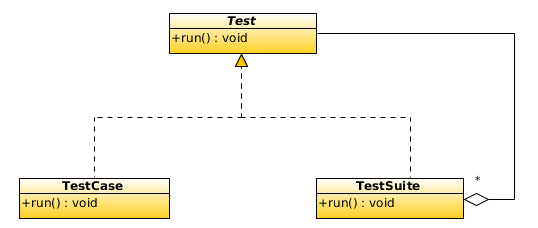
\includegraphics[width=0.8\textwidth]{figures/xunit/test-tree.png}
\caption{组合:构建隐式树}
 \label{fig:test-tree}
\end{figure}

\section{命名用例}

可以给每个\ascii{TestCase, TestSuite}命名,方便后期用例的定位与调试。

\subsection{测试用例}

\begin{leftbar}
 \begin{c++}[caption={\ttfamily{test/mars/core/TestCaseSpec.cc}}]
#include <gtest/gtest.h>
#include "mars/core/TestCase.h"

namespace {
  void assertName(const Test& test, const char* expected) {
    ASSERT_EQ(std::string(expected), test.getName());
  }
}

TEST(NamedTestCase, named_test_case) {
  assertName(TestCase("test case1"), "test case1");
}
 \end{c++}
\end{leftbar}

\subsection{通过测试}

首先,增加抽象接口\ascii{Test::getName}。

\begin{leftbar}
 \begin{c++}[caption={\ttfamily{include/mars/core/Test.h}}]
#include <string>

struct Test {
  virtual ~Test() {}
  virtual const std::string& getName() const = 0;
  virtual void run() = 0;
};
 \end{c++}
\end{leftbar}

在\ascii{TestCase}中覆写\ascii{getName}成员函数。其中,为默认构造函数提供空字符串,保证既有的用例都能通过。

\begin{leftbar}
 \begin{c++}[caption={\ttfamily{include/mars/core/TestCase.h}}]
#include "mars/core/Test.h"

struct TestCase : Test {
  explicit TestCase(const std::string& = "");

private:
  const std::string& getName() const override;
  void run() override;

private:
  virtual void setUp() {}
  virtual void runTest() {}
  virtual void tearDown() {}

private:
  std::string name;
};
 \end{c++}
\end{leftbar}

在\ascii{TestCase.cc}中实现,也极为简单。

\begin{leftbar}
 \begin{c++}[caption={\ttfamily{include/mars/core/TestCase.h}}]
#include "mars/core/TestCase.h"

TestCase::TestCase(const std::string& name) : name(name) {
}

const std::string& TestCase::getName() const {
  return name;
}

// ...
 \end{c++}
\end{leftbar}

依葫芦画瓢,\ascii{TestSuite}的名字实现与\ascii{TestCase}雷同。

\begin{leftbar}
 \begin{c++}[caption={\ttfamily{include/mars/core/TestSuite.h}}]
#include <vector>
#include "mars/core/Test.h"

struct TestSuite : Test {
  explicit TestSuite(const std::string& = "");
  ~TestSuite();

  void add(Test* test);

private:
  const std::string& getName() const override;
  void run() override;

private:
  template <typename F>
  void foreach(F f) const;

private:
  std::string name;
  std::vector<Test*> tests;
};
 \end{c++}
\end{leftbar}

\begin{leftbar}
 \begin{c++}[caption={\ttfamily{include/mars/core/TestSuite.h}}]
#include "mars/core/TestSuite.h"

TestSuite::TestSuite(const std::string& name) : name(name) {
}

const std::string& TestSuite::getName() const {
  return name;
}

// ...
 \end{c++}
\end{leftbar}

至此,测试通过。

\subsection{消除重复}

但是,\ascii{TestCase}与\ascii{TestSuite}存在结构性重复设计,包括相同的构造函数,覆写\ascii{getName}成员函数,私有字段\ascii{name}。为了消除重复,重构将公共实现搬迁至父类。

搬迁至父类需要关注两点:

\begin{enum}
  \eitem{\ascii{Test}的构造函数被声明为\ascii{public},方便子类使用\ascii{using}语句直接复用构造函数。}
  \eitem{\ascii{getName}没有必要声明为虚函数,因为在\ascii{Test}内已经完全具备实现的条件;子类强制继承\ascii{getName}的实现,拒绝被覆写。}
\end{enum}

\begin{leftbar}
 \begin{c++}[caption={\ttfamily{include/mars/core/Test.h}}]
#include <string>

struct Test {
  explicit Test(const std::string& name = "");
  const std::string& getName() const;

  virtual ~Test() {}
  virtual void run() = 0;

private:
  std::string name;
};
 \end{c++}
\end{leftbar}

\ascii{Test::getName}实现异常简单。

\begin{leftbar}
 \begin{c++}[caption={\ttfamily{src/mars/core/Test.cc}}]
#include "mars/core/Test.h"

Test::Test(const std::string& name) : name(name) {
}

const std::string& Test::getName() const {
  return name;
}
 \end{c++}
\end{leftbar}

在\ascii{TestCase}中,直接使用\ascii{using}语句复用构造函数,删除既有的\ascii{TestCase::getName}实现,及其私有字段\ascii{std::string name}。

\begin{leftbar}
 \begin{c++}[caption={\ttfamily{include/mars/core/TestCase.h}}]
#include "mars/core/Test.h"

struct TestCase : Test {
  using Test::Test;

private:
  void run() override;

private:
  virtual void setUp() {}
  virtual void runTest() {}
  virtual void tearDown() {}
};
 \end{c++}
\end{leftbar}

同理,\ascii{TestSuite}中通过相同的手段实现代码复用。

\begin{leftbar}
 \begin{c++}[caption={\ttfamily{include/mars/core/TestSuite.h}}]
#include <vector>
#include "mars/core/Test.h"

struct TestSuite : Test {
  using Test::Test;

  ~TestSuite();subsection

  void add(Testsubsection

private:
  void run() override;

private:
  template <typename F>
  void foreach(F f) const;

private:
  std::vector<Test*> tests;
};
 \end{c++}
\end{leftbar}

遗憾的是,\ascii{Test}构造函数未能声明为\ascii{protected}。但是,即使\ascii{Test}的构造函数虽然被声明为\ascii{public},设计并未丢失编译时的安全检查。因为\ascii{Test::run}被声明为纯虚函数,在编译时保证用户无法直接创建\ascii{Test}实例。

\end{content}


\begin{savequote}[45mm]
\ascii{Any fool can write code that a computer can understand. Good programmers write code that humans can understand.}
\qauthor{\ascii{- Martin Flower}}
\end{savequote}

\chapter{聚集参数} 
\label{ch:param-collector}

\begin{content}

\end{content}

\section{收集器}

\begin{content}

在之前的测试用例里,在匿名命名空间内引入计数器\ascii{num}。当某个用例被执行时,其\ascii{num++}。操作游离在对象之外的计数器是极为危险的,即使该计数器已经被限制在匿名命名空间内;因为,在其可见的作用域内都有可能被他人修改。

这是一种脆弱的设计,用户需要小心地维护计数器的初始化,也需要用户精细控制计数器累加的时机。一则容易引入不经意的错误,二则让计数器的操作散乱到各个子类覆写的\ascii{runTest}之中。

\subsection{测试用例}

为了消除这个不稳定的设计,这里引入\ascii{TestResult}的抽象,它专门负责计数器维护,及其测试结果收集等职责。重构测试用例,对外暴露\ascii{TestResult::runCount}的查询接口。

\begin{leftbar}
 \begin{c++}[caption={\ttfamily{test/mars/core/TestSuiteSpec.cc}}]
#include <gtest/gtest.h>
#include "mars/core/TestCase.h"
#include "mars/core/TestSuite.h"
#include "mars/core/TestResult.h"

namespace {
  struct TestSuiteSpec : testing::Test {
    void run(::Test& test) {
      test.run(result);
    }

  protected:
    TestResult result;
  };
}

TEST_F(TestSuiteSpec, run_multi_test_cases_using_test_suite) {
  TestSuite suite;
  suite.add(new TestCase);
  suite.add(new TestCase);

  run(suite);

  ASSERT_EQ(2, result.runCount());
}
 \end{c++}
\end{leftbar}

\subsection{实现TestResult}

\ascii{TestResult}维护了一个计数器,负责计数器初始化,累计操作数的职责。

\begin{leftbar}
 \begin{c++}[caption={\ttfamily{include/mars/core/TestResult.h}}]
struct TestResult {
  TestResult();

  void onRun();
  int runCount() const;

private:
  int numOfRuns;
};
 \end{c++}
\end{leftbar}

实现\ascii{TestResult}也较为简单。

\begin{leftbar}
 \begin{c++}[caption={\ttfamily{src/mars/core/TestResult.cc}}]
#include "mars/core/TestResult.h"

TestResult::TestResult() : numOfRuns(0) {
}

void TestResult::onRun() {
  numOfRuns++;
}

int TestResult::runCount() const {
  return numOfRuns;
}
 \end{c++}
\end{leftbar}

\subsection{重构TestCase}

当执行\ascii{TestCase::run}时,通知\ascii{TestResult}累加计数器。为了使得代码具有层次感,提取了\ascii{TestCase::runBare}的子函数,使得\ascii{TestCase::run}的主干更加清晰明了。

在头文件中,提取的\ascii{TestCase::runBare}的子函数声明为\ascii{private}。

\begin{leftbar}
 \begin{c++}[caption={\ttfamily{include/mars/core/TestCase.h}}]
#include "mars/core/Test.h"

struct TestCase : Test {
  using Test::Test;

private:
  void run(TestResult&) override;

private:
  virtual void setUp() {}
  virtual void runTest() {}
  virtual void tearDown() {}

private:
  void runBare();
};
 \end{c++}
\end{leftbar}

在实现文件中,搬迁主干逻辑至\ascii{TestCase::runBare}。

\begin{leftbar}
 \begin{c++}[caption={\ttfamily{src/mars/core/TestCase.cc}}]
#include "mars/core/TestCase.h"
#include "mars/core/TestResult.h"

void TestCase::runBare() {
  setUp();
  runTest();
  tearDown();
}

void TestCase::run(TestResult& result) {
  result.onRun();
  runBare();
}
 \end{c++}
\end{leftbar}

\subsection{重构TestSuite}

重构\ascii{TestSuite::run},每次迭代将\ascii{result}透传给\ascii{Test::run},实现多态调用。

\begin{leftbar}
 \begin{c++}[caption={\ttfamily{src/mars/core/TestSuite.cc}}]
#include "mars/core/TestSuite.h"

// ...

void TestSuite::run(TestResult& result) {
  foreach([&result](auto test) {
    test->run(result);
  });
}
 \end{c++}
\end{leftbar}

至此,测试通过。\ascii{TestResult}扮演了聚集参数的角色,它在运行时收集测试运行的结果。

\begin{figure}[H]
\centering
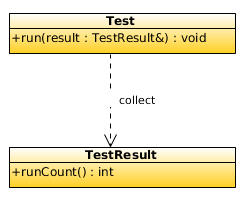
\includegraphics[width=0.4\textwidth]{figures/xunit/test-result.png}
\caption{聚集参数:收集测试结果}
 \label{fig:test-tree}
\end{figure}

\section{统计器}

\ascii{TestResult::runCount}在运行时,通过监听接口统计测试用例的数目。事实上,也可以遍历用例树,直接统计测试用例的数目。构造一个失败的用例,观察如何统计测试用例数目。

\subsection{测试用例}

\begin{leftbar}
 \begin{c++}[caption={\ttfamily{test/mars/core/TestSuiteSpec.cc}}]
#include <gtest/gtest.h>
#include "mars/core/TestCase.h"
#include "mars/core/TestSuite.h"
#include "mars/core/TestResult.h"

namespace {
  struct TestSuiteSpec : testing::Test {
    void run(::Test& test) {
      test.run(result);
    }

    int countTestCases(::Test& test) {
      return test.countTestCases();
    }

  protected:
    TestResult result;
  };
}

TEST_F(TestSuiteSpec, run_multi_test_cases_using_test_suite) {
  TestSuite suite;
  suite.add(new TestCase);
  suite.add(new TestCase);

  run(suite);

  ASSERT_EQ(2, countTestCases(suite));
}
 \end{c++}
\end{leftbar}

\subsection{定义虚接口}

增加\ascii{Test::countTestCases}纯虚接口。

\begin{leftbar}
 \begin{c++}[caption={\ttfamily{include/mars/core/Test.h}}]
#include <string>

struct TestResult;

struct Test {
  explicit Test(const std::string& name = "");
  const std::string& getName() const;

  virtual ~Test() {}
  virtual int countTestCases() const = 0;
  virtual void run(TestResult&) = 0;

private:
  std::string name;
};
 \end{c++}
\end{leftbar}

\subsection{实现虚接口}

\ascii{TestCase::countTestCases}覆写行为直接返回\ascii{1}。

\begin{leftbar}
 \begin{c++}[caption={\ttfamily{src/mars/core/TestCase.cc}}]
int TestCase::countTestCases() const {
  return 1;
}
 \end{c++}
\end{leftbar}

\ascii{TestSuite::countTestCases}覆写行为完成\ascii{reduce}操作。

\begin{leftbar}
 \begin{c++}[caption={\ttfamily{src/mars/core/TestSuite.cc}}]
int TestSuite::countTestCases() const {
  auto num = 0;
  foreach([&num](auto test) {
    num += test->countTestCases();
  });
  return num;
}
 \end{c++}
\end{leftbar}

至此,测试通过。相对于\ascii{TestResult::runCount}通过聚集参数实现用例数目的统计,\ascii{TestResult::countTestCases}更加具有可扩展性;并且,\ascii{TestResult}与\ascii{TestCase}的耦合程度更小。

\end{content}


% \begin{savequote}[45mm]
\ascii{Any fool can write code that a computer can understand. Good programmers write code that humans can understand.}
\qauthor{\ascii{- Martin Flower}}
\end{savequote}

\chapter{异常处理} 
\label{ch:except-handle}

\begin{content}

\end{content}

\section{断言失败}

\begin{content}

至此,框架不能处理任何异常逻辑。当用户调用\ascii{ASSERT\_EQ}失败时,抛出\ascii{AssertionError}异常,框架捕获该异常,标记该测试用例为\ascii{Failure};如果抛出其他异常,并被\ascii{mars}框架捕获,则标记该测试用例为\ascii{Error}。显式区分这两种异常类型,使得用户可以审查自己的测试用例,并修复失败的用例。

\subsection{测试用例}

当用例的断言失败,打印诸如如下详细信息,提示用户修复失败的用例。

\begin{leftbar}
 \begin{python}[caption={测试失败}]
/home/horance/code/cpp/mars/test/mars/core/TestCaseSpec.cc:33
expected value == 2, but got 0
 \end{python}
\end{leftbar}

接下来,构建失败的用例,在\ascii{runTest}时抛出异常\ascii{AssertionError},模拟断言失败的场景。

\begin{leftbar}
 \begin{c++}[caption={\ttfamily{test/mars/TestCaseSpec.cc}}]
#include <gtest/gtest.h>
#include "mars/core/TestCase.h"
#include "mars/except/AssertionError.h"

namespace {
  struct TestCaseSpec : testing::Test {
  protected:
    void run(::Test& test) {
      test.run(result);
    }

  protected:
    TestResult result;
  };

  struct AssertionFailedTest : TestCase {
    void runTest() override {
      throw AssertionError("test.cpp:57", "expected value == 2, but got 3");
    }
  };
}

TEST_F(TestCaseSpec, throw_assertion_error_on_run_test) {
  AssertionFailedTest test;
  run(test);

  ASSERT_EQ(1, result.failCount());
}
 \end{c++}
\end{leftbar}

\subsection{异常类}

为了通过编译,引入\ascii{AssertionError}的异常类。它携带了断言失败处的文件名与行号\ascii{(src)},及其用例断言失败的具体原因\ascii{(msg)}。

\begin{leftbar}
 \begin{c++}[caption={\ttfamily{include/mars/except/AssertionError.h}}]
#include <string>
#include <exception>

struct AssertionError : std::exception {
  AssertionError(const std::string& src, const std::string& msg);
  ~AssertionError() noexcept = default;

  const char* what() const noexcept;

private:
  std::string msg;
};
 \end{c++}
\end{leftbar}

\ascii{AssertionError}实现如下。

\begin{leftbar}
 \begin{c++}[caption={\ttfamily{src/mars/except/AssertionError.cc}}]
#include "mars/except/AssertionError.h"

AssertionError::AssertionError(const std::string& src,
  const std::string& msg) : msg(src + "\n" + msg) {
}

const char* AssertionError::what() const noexcept {
  return msg.c_str();
}
 \end{c++}
\end{leftbar}

\subsection{失败计数器}

\ascii{TestResult}新增名为\ascii{numOfFails}的计数器。

\begin{leftbar}
 \begin{c++}[caption={\ttfamily{include/mars/core/TestResult.h}}]
struct TestResult {
  TestResult();

  int failCount() const;
  void onFail();

private:
  int numOfFails;
};
 \end{c++}
\end{leftbar}

在实现文件中,实现失败计数器的初始化,累加,与查询逻辑。

\begin{leftbar}
 \begin{c++}[caption={\ttfamily{src/mars/core/TestResult.cc}}]
#include "mars/core/TestResult.h"

TestResult::TestResult() : numOfFails(0) {
}

int TestResult::failCount() const {
  return numOfFails;
}

void TestResult::onFail() {
  numOfFails++;
}
 \end{c++}
\end{leftbar}

\subsection{捕获异常}

当执行\ascii{TestCase::run}时,捕获异常并通过调用\ascii{TestResult::fail},累加计数器\ascii{numOfFails}。

\begin{leftbar}
 \begin{c++}[caption={\ttfamily{src/mars/core/TestCase.cc}}]
#include "mars/core/TestCase.h"
#include "mars/core/TestResult.h"
#include "mars/except/AssertionError.h"

void TestCase::run(TestResult& result) {
  setUp();

  try {
    runTest();
  } catch (const AssertionError&) {
    result.onFail();
  }

  tearDown();
}

// ...
 \end{c++}
\end{leftbar}

至此,测试通过。

\section{前置失败}

\ascii{TestCase}执行时,还未执行至\ascii{runTest}时,执行\ascii{setUp}可能就提前失败了。

\subsection{测试用例}

构建失败的用例,模拟前置失败的场景。

\begin{leftbar}
 \begin{c++}[caption={\ttfamily{test/mars/TestCaseSpec.cc}}]
namespace {
  struct AssertionFailedOnSetUpTest : TestCase {
    bool wasRun = false;

  private:
    void setUp() override {
      throw AssertionError("test.cpp:57", "expected value == 2, but got 3");
    }

    void runTest() override {
      wasRun = true;
    }
  };
}

TEST_F(TestCaseSpec, throw_assertion_error_on_setup) {
  AssertionFailedOnSetUpTest test;
  run(test);

  ASSERT_EQ(1, result.failCount());
  ASSERT_FALSE(test.wasRun);
}
 \end{c++}
\end{leftbar}

\subsection{捕获异常}

为了通过测试,当执行\ascii{TestCase::setUp}时,捕获异常并通知\ascii{TestResult},然后立即终止用例的执行;毕竟环境没准备好,强制执行用例毫无意义。

\begin{leftbar}
 \begin{c++}[caption={\ttfamily{src/mars/core/TestCase.cc}}]
#include "mars/core/TestCase.h"
#include "mars/core/TestResult.h"
#include "mars/except/AssertionError.h"

void TestCase::run(TestResult& result) {
  bool succ = false;
  try {
    setUp();
    succ = true;
  } catch (const AssertionError&) {
    result.onFail();
  }

  if (succ) {
    try {
      runTest();
    } catch (const AssertionError&) {
      result.onFail();
    }
  }

  tearDown();
}
 \end{c++}
\end{leftbar}

至此,测试通过。

\section{后置失败}

\ascii{TestCase::runBare}执行时,执行完\ascii{setUp, runTest}成功之后,接着执行\ascii{tearDown}时失败。

\subsection{测试用例}

构建失败的用例,模拟后置失败的场景。

\begin{leftbar}
 \begin{c++}[caption={\ttfamily{test/mars/TestCaseSpec.cc}}]
namespace {
  struct AssertionFailedOnTearDownTest : TestCase {
    void tearDown() override {
      throw AssertionError("test.cpp:57", "expected value == 2, but got 3");
    }
  };
}

TEST_F(TestCaseSpec, throw_assertion_error_on_tear_down) {
  AssertionFailedOnTearDownTest test;
  run(test);

  ASSERT_EQ(1, result.failCount());
}
 \end{c++}
\end{leftbar}

\subsection{捕获异常}

当执行\ascii{TestCase::tearDown}时,捕获异常并通知\ascii{TestResult}。但是,无论\ascii{setUp, runTest}成败与否,\ascii{tearDown}都要强制执行,保证资源的安全释放。

\begin{leftbar}
 \begin{c++}[caption={\ttfamily{src/mars/core/TestCase.cc}}]
#include "mars/core/TestCase.h"
#include "mars/core/TestResult.h"
#include "mars/except/AssertionError.h"

void TestCase::run(TestResult& result) {
  bool succ = false;
  try {
    setUp();
    succ = true;
  } catch (const AssertionError&) {
    result.onFail();
  }

  if (succ) {
    try {
      runTest();
    } catch (const AssertionError&) {
      result.onFail();
    }
  }

  try {
    tearDown();
  } catch (const AssertionError&) {
    result.onFail();
  }
}
 \end{c++}
\end{leftbar}

至此,测试通过。

\section{错误:抛出std::exception}

当抛出\ascii{AssertionError},称之为\ascii{Failure};当抛出其他异常,称之为\ascii{Error}。

\subsection{测试用例}

构建失败的用例,模拟其他异常抛出的场景。

\begin{leftbar}
 \begin{c++}[caption={\ttfamily{test/mars/TestCaseSpec.cc}}]
namespace {
  struct StdExceptionTest : TestCase {
    void runTest() override {
      throw std::exception();
    }
  };
}

TEST_F(TestCaseSpec, throw_std_exception_on_run_test) {
  StdExceptionTest test;
  run(test);

  ASSERT_EQ(0, result.failCount());
  ASSERT_EQ(1, result.errorCount());
}
 \end{c++}
\end{leftbar}

\subsection{错误计数器}

增加查询函数\ascii{TestResult::errorCount}查询函数,错误监听接口\ascii{TestResult::onError},及其相应的错误计数器\ascii{numOfErrors}。

\begin{leftbar}
 \begin{c++}[caption={\ttfamily{include/mars/core/TestResult.h}}]
struct TestResult {
  TestResult();

  int failCount() const;
  int errorCount() const;

  void onFail();
  void onError();

private:
  int numOfFails;
  int numOfErrors;
};
 \end{c++}
\end{leftbar}

在实现文件中,依葫芦画瓢,实现\ascii{TestResult::errorCount, TestResult::onError}。

\begin{leftbar}
 \begin{c++}[caption={\ttfamily{src/mars/core/TestResult.cc}}]
#include "mars/core/TestResult.h"

TestResult::TestResult()
  : numOfFails(0), numOfErrors(0) {
}

int TestResult::failCount() const {
  return numOfFails;
}

int TestResult::errorCount() const {
  return numOfErrors;
}

void TestResult::onFail() {
  numOfFails++;
}

void TestResult::onError() {
  numOfErrors++;
}
 \end{c++}
\end{leftbar}

\subsection{捕获异常}

当执行\ascii{TestCase::runTest}时,捕获\ascii{std::exception}异常,并通知\ascii{TestResult::error}累加计数器。

\begin{leftbar}
 \begin{c++}[caption={\ttfamily{src/mars/core/TestCase.cc}}]
#include "mars/core/TestCase.h"
#include "mars/core/TestResult.h"
#include "mars/except/AssertionError.h"

void TestCase::run(TestResult& result) {
  bool succ = false;
  try {
    setUp();
    succ = true;
  } catch (const AssertionError&) {
    result.onFail();
  }

  if (succ) {
    try {
      runTest();
    } catch (const AssertionError&) {
      result.onFail();
    } catch (const std::exception&) {
      result.onError();
    }
  }

  try {
    tearDown();
  } catch (const AssertionError&) {
    result.onFail();
  }
}
 \end{c++}
\end{leftbar}

\section{未知错误}

当抛出其他未知的异常,测试框架需要捕获,并标记为\ascii{Error},提示用户被测系统存在严重的漏洞。

\subsection{测试用例}

\begin{leftbar}
 \begin{c++}[caption={\ttfamily{test/mars/TestCaseSpec.cc}}]
namespace {
  struct UnknownException {};

  struct UnknownExceptionTest : TestCase {
    void runTest() override {
      throw UnknownException();
    }
  };
}

TEST_F(TestCaseSpec, throw_unknown_exception_on_run_test) {
  UnknownExceptionTest test;
  run(test);

  ASSERT_EQ(0, result.failCount());
  ASSERT_EQ(1, result.errorCount());
}
 \end{c++}
\end{leftbar}

\subsection{捕获异常}

当执行\ascii{TestCase::runTest}时,捕获未知的异常,并通知\ascii{TestResult::error}累加计数器。

\begin{leftbar}
 \begin{c++}[caption={\ttfamily{src/mars/core/TestCase.cc}}]
#include "mars/core/TestCase.h"
#include "mars/core/TestResult.h"
#include "mars/except/AssertionError.h"

void TestCase::run(TestResult& result) {
  bool succ = false;
  try {
    setUp();
    succ = true;
  } catch (const AssertionError&) {
    result.onFail();
  }

  if (succ) {
    try {
      runTest();
    } catch (const AssertionError&) {
      result.onFail();
    } catch (const std::exception&) {
      result.onError();
    } catch (...) {
      result.onError();
    }    
  }

  try {
    tearDown();
  } catch (const AssertionError&) {
    result.onFail();
  }
}
 \end{c++}
\end{leftbar}

测试通过。

\section{完备的异常处理}

依次构建测试用例,小步快走,驱动出完备的异常处理逻辑。

\begin{leftbar}
 \begin{c++}[caption={\ttfamily{src/mars/core/TestCase.cc}}]
#include "mars/core/TestCase.h"
#include "mars/core/TestResult.h"
#include "mars/except/AssertionError.h"

void TestCase::run(TestResult& result) {
  bool succ = false;
  try {
    setUp();
    succ = true;
  } catch (const AssertionError&) {
    result.onFail();
  } catch (const std::exception&) {
    result.onError();
  } catch (...) {
    result.onError();
  }

  if (succ) {
    try {
      runTest();
    } catch (const AssertionError&) {
      result.onFail();
    } catch (const std::exception&) {
      result.onError();
    } catch (...) {
      result.onError();
    }
  }

  try {
    tearDown();
  } catch (const AssertionError&) {
    result.onFail();
  } catch (const std::exception&) {
    result.onError();
  } catch (...) {
    result.onError();
  }
}

// ...
 \end{c++}
\end{leftbar}

\ascii{TestCase::run}实现不仅存在重复逻辑,而且异常臃肿,异常丑陋。此时不重构,更待何时。

\subsection{消除重复}

观察\ascii{TestCase::setUp, TestCase::runTest, TestCase::tearDown}的共性,它们拥有相同的函数签名,可以使用指向成员函数的指针挖掘它们的共性。

\begin{leftbar}
 \begin{c++}
using Method = void(TestCase::*)();
 \end{c++}
\end{leftbar}

提取公共函数\ascii{TestCase::protect},它返回\ascii{bool}类型。首先,在头文件中声明私有函数\ascii{TestCase::protect}。

\begin{leftbar}
 \begin{c++}[caption={\ttfamily{include/mars/core/TestCase.h}}]
#include "mars/core/Test.h"

struct TestCase : Test {
  using Test::Test;

private:
  int countTestCases() const override;
  void run(TestResult&) override;

private:
  virtual void setUp() {}
  virtual void runTest() {}
  virtual void tearDown() {}

private:
  using Method = void(TestCase::*)();
  bool protect(TestResult& result, Method method);
};
 \end{c++}
\end{leftbar}

在实现文件中,实现异常处理逻辑的代码复用。

\begin{leftbar}
 \begin{c++}[caption={\ttfamily{src/mars/core/TestCase.cc}}]
#include "mars/core/TestCase.h"
#include "mars/core/TestResult.h"
#include "mars/except/AssertionError.h"

bool TestCase::protect(TestResult& result, Method method) {
  bool succ = false;
  try {
    (this->*method)();
    succ = true;
  } catch (const AssertionError&) {
    result.onFail();
  } catch (const std::exception&) {
    result.onError();
  } catch (...) {
    result.onError();
  }
  return succ;
}

void TestCase::run(TestResult& result) {
  if (protect(result, &TestCase::setUp)) {
    protect(result, &TestCase::runTest);
  }
  protect(result, &TestCase::tearDown);
}

int TestCase::countTestCases() const {
  return 1;
}
 \end{c++}
\end{leftbar}

\end{content}


% \begin{savequote}[45mm]
\ascii{Any fool can write code that a computer can understand. Good programmers write code that humans can understand.}
\qauthor{\ascii{- Martin Flower}}
\end{savequote}

\chapter{解耦合} 
\label{ch:decoupling}

\begin{content}

\end{content}

\section{关键抽象}

\begin{content}

分析\ascii{TestCase::protect}实现,它间接调用\ascii{TestCase}的成员函数\ascii{setUp, runTest, tearDown},而异常处理逻辑主要分布于\ascii{TestResult}的成员函数\ascii{addFailure, addError}。从代码职责分布看,\ascii{TestCase::protect}主要完成异常处理逻辑,与\ascii{TestResult}关系更加紧密。

\begin{nodiff}{src/mars/core/TestCase.cc}
 \begin{c++}
#include <mars/core/TestCase.h>
#include <mars/core/TestResult.h>
#include <mars/except/AssertionError.h>

bool TestCase::protect(TestResult& result, Method method) {
  bool succ = false;
  try {
    (this->*method)();
    succ = true;
  } catch (const AssertionError&) {
    result.addFailure();
  } catch (const std::exception&) {
    result.addError();
  } catch (...) {
    result.addError();
  }
  return succ;
}

void TestCase::run(TestResult& result) {
  if (protect(result, &TestCase::setUp)) {
    protect(result, &TestCase::runTest);
  }
  protect(result, &TestCase::tearDown);
}
 \end{c++}
\end{nodiff}

根据迪米特法则,这段异常处理的逻辑应搬迁至\ascii{TestResult}。当捕获异常后,直接更新到自己的私有数据域,实现\ascii{TestResult::addFailure, TestResult::addError}监听接口的私有化。但是,如果搬迁\ascii{protect}逻辑到\ascii{TestResult},那么\ascii{TestResult}如何调用到\ascii{TestCase}的成员函数\ascii{setUp, runTest, tearDown}呢?

此时似乎陷入窘境,因为\ascii{TestCase}与\ascii{TestResult}之间的耦合太过紧密,拆分显得不是那么容易。因此,解除\ascii{TestCase}与\ascii{TestResult}之间的耦合迫在眉睫。

\subsection{函数式接口}

为了彻底解开\ascii{protect}对\ascii{TestCase}的依赖,引入关键抽象\ascii{TestCaseFunctor},相对\ascii{TestCase::Method}的简单抽象,它不包含\ascii{TestCase}的任何信息,可以与之彻底解耦。因此,\ascii{TestCaseFunctor}更加稳定、更加具有可扩展性\footnote{例如,通过增加\ascii{getTestName}接口,可以携带更多元数据。}。

\ascii{using}或\ascii{typedef}的别名机制,功能单一,抽象能力有限。最重要的是,此处它强度依赖于\ascii{TestCase}的类型信息,两者存在隐式的耦合关系。

\begin{diff}{include/mars/core/internal/TestCaseFunctor.h}
 \begin{minicpp}
using Method = void(TestCase::*)();
 \end{minicpp}
\tcblower
 \begin{minicpp}
struct TestCaseFunctor {
  virtual bool operator()() const = 0;
  virtual ~TestCaseFunctor() {}
};
 \end{minicpp}
\end{diff}

\subsection{实现抽象}

在\ascii{TestCase.h}的文件中,修改\ascii{TestCase::protect}的声明,让其依赖于更稳定的抽象\ascii{TestCaseFunctor},而非简单抽象\ascii{TestCase::Method}。

\begin{diff}{include/mars/core/TestCase.h}
 \begin{minicpp}
#include <mars/core/Test.h>
#include <mars/core/TestFixture.h>

struct TestCase : Test, private TestFixture {
  using Test::Test;

private:
  void run(TestResult&) override;
  int countTestCases() const override;

private:
  virtual void runTest() {}

private:
  using Method = void(TestCase::*)();
  bool protect(TestResult& result, Method method);
};
 \end{minicpp}
\tcblower
 \begin{minicpp}
#include <mars/core/Test.h>
#include <mars/core/TestFixture.h>

struct TestCaseFunctor;

struct TestCase : Test, private TestFixture {
  using Test::Test;

private:
  void run(TestResult&) override;
  int countTestCases() const override;

private:
  virtual void runTest() {}

private:
  bool protect(TestResult&, const TestCaseFunctor&);
}; 
  \end{minicpp}
\end{diff}

在\ascii{TestCase.cc}实现文件中,在匿名命名空间内定义实现\ascii{Functor},它是\ascii{TestCaseFunctor}背后运行的真正实现,它封装实现了原来\ascii{TestCase::Method}的间接调用。

\begin{diff}{src/mars/core/TestCase.cc}
 \begin{minicpp}
#include <mars/core/TestCase.h>
#include <mars/core/TestResult.h>
#include <mars/except/AssertionError.h>

bool TestCase::protect
  (TestResult& result, Method method) {
  bool succ = false;
  try {
    (this->*method)();
    succ = true;
  } catch (const AssertionError&) {
    result.addFailure();
  } catch (const std::exception&) {
    result.addError();
  } catch (...) {
    result.addError();
  }
  return succ;
}

void TestCase::run(TestResult& result) {
  if (protect(result, &TestCase::setUp)) {
    protect(result, &TestCase::runTest);
  }
  protect(result, &TestCase::tearDown);
}
 \end{minicpp}
\tcblower
 \begin{minicpp}
#include <mars/core/TestCase.h>
#include <mars/core/TestResult.h>
#include <mars/except/AssertionError.h>
#include <mars/core/internal/TestCaseFunctor.h>

namespace {
  struct Functor : TestCaseFunctor {
    using Method = void(TestCase::*)();

    Functor(TestCase* self, Method method)
      : self(self), method(method) {
    }

  private:
    bool operator()() const override {
      (self->*method)();
      return true;
    }

  private:
    TestCase* self;
    Method method;
  };
}

bool TestCase::protect
  (TestResult& result, const TestCaseFunctor& f) {
  try {
    return f();
  } catch (const AssertionError&) {
    result.addFailure();
  } catch (const std::exception&) {
    result.addError();
  } catch (...) {
    result.addError();
  }
  return false;
}

void TestCase::run(TestResult& result) {
  if (protect(result, Functor(this, &TestCase::setUp))) {
    protect(result, Functor(this, &TestCase::runTest));
  }
  protect(result, Functor(this, &TestCase::tearDown));
}
  \end{minicpp}
\end{diff}

经验证测试是通过的,重构是成功的。

\end{content}

\section{搬迁逻辑}

\begin{content}

\subsection{重构TestResult}

运用迪米特法则,将异常处理的逻辑从\ascii{TestCase::protect}搬迁至\ascii{TestResult::protect}。因为\ascii{TestResult::protect}依赖于\ascii{TestCaseFunctor}的抽象类型,而非具体的\ascii{TestCase},实现了\ascii{TestResult::protect}对\ascii{TestCase}的解耦。

在头文件\ascii{TestResult.h}中,公开\ascii{TestResult::protect},而私有\ascii{TestResult::addFailure, TestResult::addError}。

\begin{diff}{include/mars/core/TestResult.h}
 \begin{minicpp}
struct TestResult {
  TestResult();

  void addFailure();
  int failCount() const;

  void addError();
  int errorCount() const;

private:
  int numOfFails;
  int numOfErrors;
};
 \end{minicpp}
\tcblower 
 \begin{minicpp}
struct TestCaseFunctor;

struct TestResult {
  TestResult();

  int failCount() const;
  int errorCount() const;

  bool protect(const TestCaseFunctor&);

private:
  void addFailure();
  void addError();

private:
  int numOfFails;
  int numOfErrors;
};
 \end{minicpp}
\end{diff}

在实现文件中,搬迁\ascii{TestCase::protect}的异常处理逻辑至此处。此时,切忌不要提前删除\ascii{TestCase::protect}的逻辑。

\begin{diff}{src/mars/core/TestResult.cc}
 \begin{minicpp}
#include <mars/core/TestResult.h>

TestResult::TestResult()
  : numOfFails(0), numOfErrors(0) {
}

int TestResult::failCount() const {
  return numOfFails;
}

int TestResult::errorCount() const {
  return numOfErrors;
}

void TestResult::addFailure() {
  numOfFails++;
}

void TestResult::addError() {
  numOfErrors++;
}
 \end{minicpp}
\tcblower 
 \begin{minicpp}
#include <mars/core/TestResult.h>
#include <mars/except/AssertionError.h>
#include <mars/core/internal/TestCaseFunctor.h>

TestResult::TestResult()
  : numOfFails(0), numOfErrors(0) {
}

int TestResult::failCount() const {
  return numOfFails;
}

int TestResult::errorCount() const {
  return numOfErrors;
}

inline void TestResult::addFailure() {
  numOfFails++;
}

inline void TestResult::addError() {
  numOfErrors++;
}

bool TestResult::protect(const TestCaseFunctor& f) {
  try {
    return f();
  } catch (const AssertionError&) {
    addFailure();
  } catch (const std::exception&) {
    addError();
  } catch (...) {
    addError();
  }
  return false;
}
 \end{minicpp}
\end{diff}

\subsection{重构TestCase}

重构\ascii{TestCase::run},使其调用\ascii{TestResult::protect}。测试通过后,最后安全地删除既有的\ascii{TestCase::protect}实现,至此完成了\ascii{protect}逻辑从\ascii{TestCase}到\ascii{TestResult}的搬迁过程,重构完毕。

\begin{diff}{src/mars/core/TestCase.cc}
 \begin{minicpp}
#include <mars/core/TestCase.h>
#include <mars/core/TestResult.h>
#include <mars/except/AssertionError.h>
#include <mars/core/internal/TestCaseFunctor.h>

namespace {
  struct Functor : TestCaseFunctor {
    using Method = void(TestCase::*)();

    Functor(TestCase* self, Method method)
      : self(self), method(method) {
    }

  private:
    bool operator()() const override {
      (self->*method)();
      return true;
    }

  private:
    TestCase* self;
    Method method;
  };
}

bool TestCase::protect
  (TestResult& result, const TestCaseFunctor& f) {
  try {
    return f();
  } catch (const AssertionError&) {
    result.addFailure();
  } catch (const std::exception&) {
    result.addError();
  } catch (...) {
    result.addError();
  }
  return false;
}

void TestCase::run(TestResult& result) {
  if (protect(result, Functor(this, &TestCase::setUp))) {
    protect(result, Functor(this, &TestCase::runTest));
  }
  protect(result, Functor(this, &TestCase::tearDown));
}
 \end{minicpp}
\tcblower 
 \begin{minicpp}
#include <mars/core/TestCase.h>
#include <mars/core/TestResult.h>
#include <mars/core/internal/TestCaseFunctor.h>

namespace {
  struct Functor : TestCaseFunctor {
    using Method = void(TestCase::*)();

    Functor(TestCase* self, Method method)
      : self(self), method(method) {
    }

  private:
    bool operator()() const override {
      (self->*method)();
      return true;
    }

  private:
    TestCase* self;
    Method method;
  };
}

void TestCase::run(TestResult& result) {
  if (result.protect(Functor(this, &TestCase::setUp))) {
    result.protect(Functor(this, &TestCase::runTest));
  }
  result.protect(Functor(this, &TestCase::tearDown));
}
 \end{minicpp}
\end{diff}

\subsubsection{改善表达力}

可以定义一个宏,改善\ascii{TestCase::run}对\ascii{TestResult::protect}调用的表达力。不忘初心,\ascii{TestCase::run}算法主干回归至最开始的简单逻辑。

\begin{diff}{src/mars/core/TestCase.cc}
 \begin{minicpp}
void TestCase::run(TestResult& result) {
  if (result.protect(Functor(this, &TestCase::setUp))) {
    result.protect(Functor(this, &TestCase::runTest));
  }
  result.protect(Functor(this, &TestCase::tearDown));
}
 \end{minicpp}
\tcblower 
 \begin{minicpp}
#define PROTECT(method) \
  result.protect(Functor(this, &TestCase::method))

void TestCase::run(TestResult& result) {
  if (PROTECT(setUp)) {
    PROTECT(runTest);
  }
  PROTECT(tearDown);
}
 \end{minicpp}
\end{diff}

\subsection{重构回顾}

在重构之前,在\ascii{TestCase}中实现异常处理逻辑\ascii{TestCase::protect}。但是,当捕获异常之后,需要调用两个公开的\ascii{TestResult::addFailure, TestResult::addError},缓存异常信息到\ascii{TestResult}本地。导致\ascii{TestCase::protect}的实现,严重依赖于\ascii{TestResult}缓存异常信息的具体实现。

\begin{figure}[H]
\centering
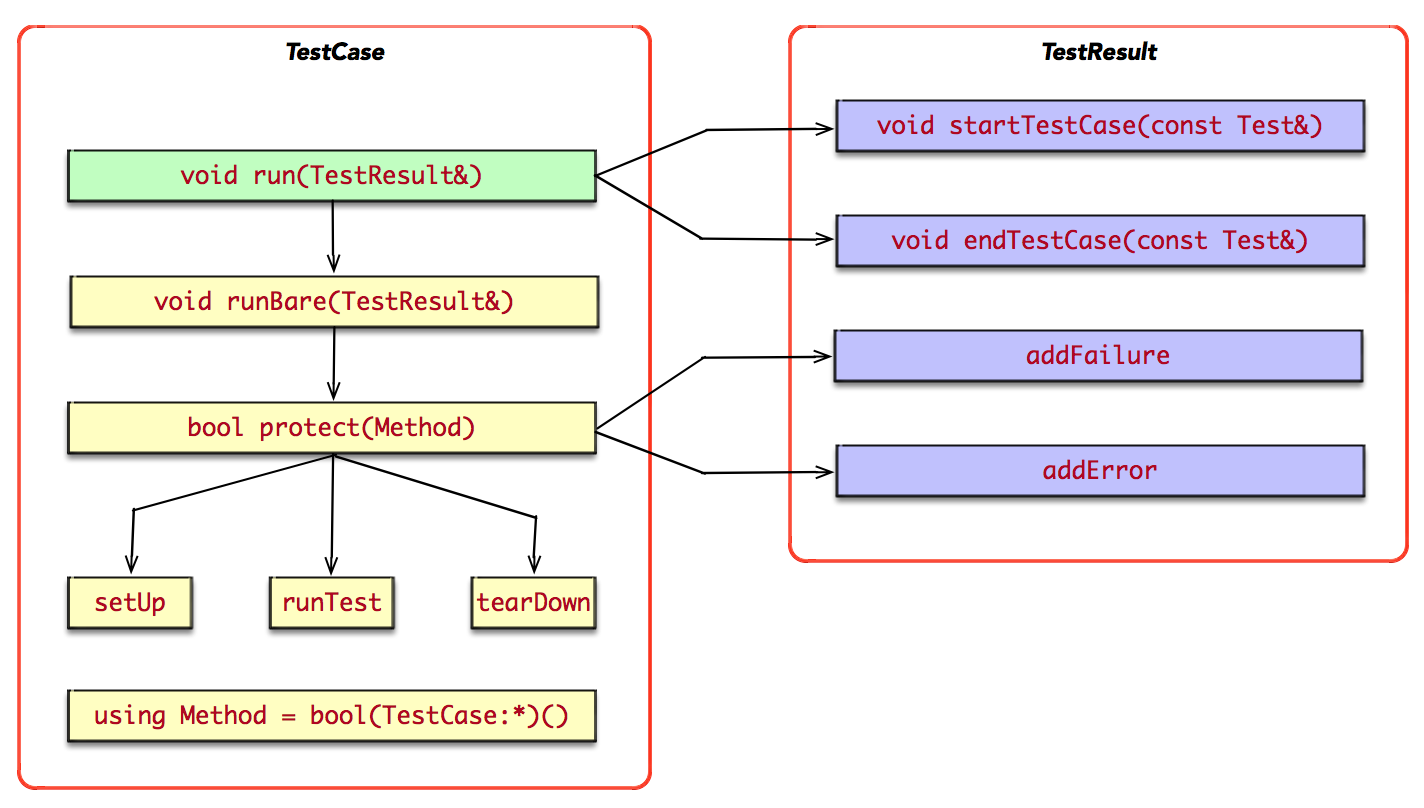
\includegraphics[width=1.0\textwidth]{figures/xunit/coupling-1.png}
\caption{重构之前}
 \label{fig:coupling-1}
\end{figure}

根据迪米特法则,将\ascii{TestCase::protect}搬迁至\ascii{TestResult::protect}。一方面,\ascii{TestResult}暴露给\ascii{TestCase}接口由\ascii{2}减少至\ascii{1},缓解了\ascii{TestCase}对\ascii{TestResult}的耦合关系。另一方面,实现\ascii{TestResult::addFailure, TestResult::addError}的私有化,使得\ascii{TestResult}取得更好的封装特性。

\begin{figure}[H]
\centering
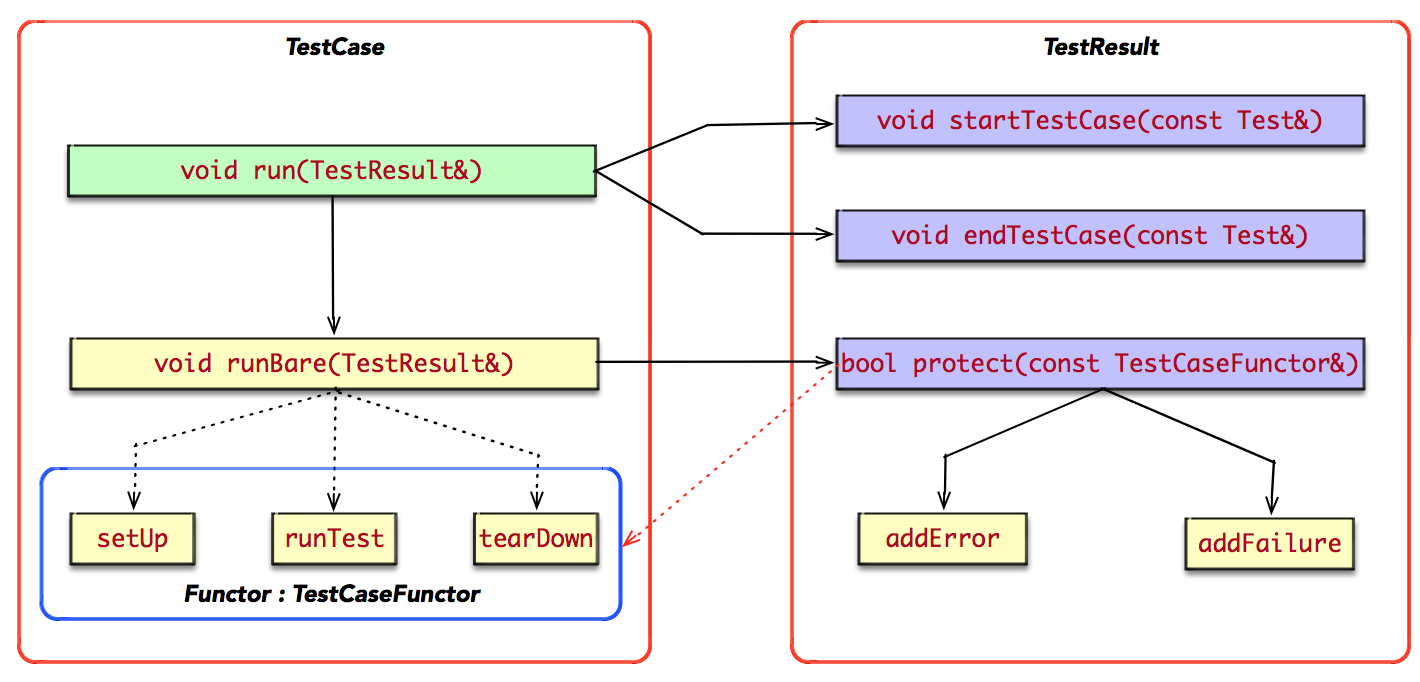
\includegraphics[width=1.0\textwidth]{figures/xunit/decoupling-1-1.png}
\caption{重构之后}
 \label{fig:decoupling-1-1}
\end{figure}

解耦的关键在于抽象接口\ascii{TestCaseFunctor}。在没有破坏\ascii{TestCase}既有封装特性的前提下,使得\ascii{TestResult::protect}不再依赖于具体的\ascii{TestCase::setup, TestCase::runTest, TestCase::tearDown}。

\begin{figure}[H]
\centering
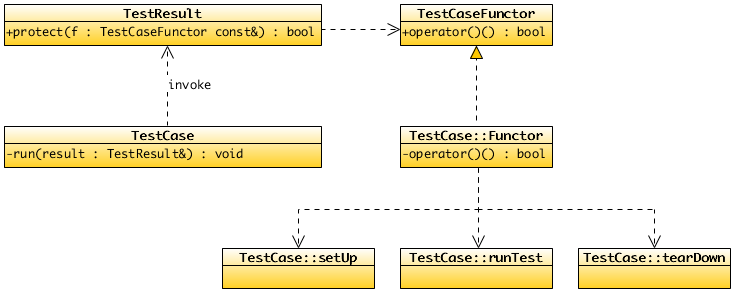
\includegraphics[width=1.0\textwidth]{figures/xunit/test-case-functor-1.png}
\caption{关键抽象: TestCaseFunctor}
 \label{fig:test-case-functor-1}
\end{figure}

\end{content}

% \section{彻底解耦}

% \begin{content}

% 宏函数\ascii{PROTECT}提高了\ascii{TestCase::run}主干逻辑的表达力,但是没有掩盖\ascii{TestCase::run}的主干逻辑与\ascii{TestResult}更亲密的基本事实真相。按照迪米特法则,\ascii{TestCase::run}的主干逻辑应该搬迁至\ascii{TestResult},使得\ascii{TestCase::protect}私有化。

% \subsection{关键抽象}

% \subsubsection{抽象接口:TestCaseProtector}

% \begin{nodiff}
%  \begin{c++}
% struct TestCaseFunctor;

% struct TestCaseProtector {
%   virtual bool protect(const TestCaseFunctor&) = 0;
%   virtual ~TestCaseProtector() {}
% }; 
%  \end{c++}
% \end{nodiff}

% \subsubsection{抽象接口:BareTestCase}

% \begin{nodiff}
%  \begin{c++}
% struct TestCaseProtector;

% struct BareTestCase {
%   virtual void runBare(TestCaseProtector&) = 0;
%   virtual ~BareTestCase() {}
% };
%  \end{c++}
% \end{nodiff}

% \end{content}




% \begin{savequote}[45mm]
\ascii{Any fool can write code that a computer can understand. Good programmers write code that humans can understand.}
\qauthor{\ascii{- Martin Flower}}
\end{savequote}

\chapter{异常信息} 
\label{ch:except-msg}

\begin{content}

\end{content}

\section{异常信息}

\begin{content}

当用例失败后,用户期望终端打印如下信息,方便用户快速修复失败的用例。

\begin{leftbar}
 \begin{c++}
assertion fail in the runTest
/home/horance/code/cpp/cut/test/hamcrest/core/ComparatorTest.cpp:12
Expected: a value eq <254: int>
     but: <255: int> eq <254: int> got false
 \end{c++}
\end{leftbar}

异常信息包括如下几个重要逻辑信息:

\begin{enum}
  \eitem{\ascii{Why}: 指明用例失败的原因}
    \begin{enum}
      \eitem{\ascii{assertion fail}: 断言失败}
      \eitem{\ascii{uncaught std::exception}: 被测系统抛出\ascii{std::exception}或子异常}
      \eitem{\ascii{uncaught unknown exception}: 被测系统抛出其他未知异常}
    \end{enum}
  \eitem{\ascii{Where}: 异常抛出的地点}
    \begin{enum}
      \eitem{\ascii{in the setUp}}
      \eitem{\ascii{in the runTest}}
      \eitem{\ascii{in the tearDown}}
    \end{enum}
  \eitem{\ascii{What}: 异常携带的详细信息}
    \begin{enum}
      \eitem{\ascii{源文件}}
      \eitem{\ascii{行号}}
      \eitem{\ascii{异常详细信息}: \ascii{what}成员函数返回值}
    \end{enum}
\end{enum}

\end{content}

\section{断言失败}

\begin{content}

\subsection{测试用例}

重构既有的测试用例,当\ascii{runTest}因断言失败而抛出\ascii{AssertionError}异常时,在\ascii{TestResult}收集异常信息。

\begin{leftbar}
 \begin{c++}[caption={\ttfamily{test/mars/core/TestCaseSpec.cc}}]
namespace {
  struct AssertionFailedTest : TestCase {
    const char* expectMsg() const {
      return "assertion fail in the runTest\n"
             "TestCaseSpec.cpp:57\n"
             "expected value == 2, but got 3";
    }

  private:
    void runTest() override {
      throw AssertionError("TestCaseSpec.cpp:57", "expected value == 2, but got 3");
    }
  };
}

TEST_F(TestCaseSpec, throw_assertion_error_on_run_test) {
  AssertionFailedTest test;
  run(test);

  auto& fails = result.getFailures(); 
  ASSERT_EQ(1, fails.size());
  ASSERT_EQ(test.expectMsg(), fails[0]);
}
 \end{c++}
\end{leftbar}

\subsection{缓存异常}

为了快速通过测试,对外提供\ascii{getFailures}查询接口,供外部用户获取异常信息。实现较为简单,在\ascii{TestResult}建立相应的数据结构,完成异常信息的收集。

\begin{leftbar}
 \begin{c++}[caption={\ttfamily{include/mars/core/TestResult.h}}]
#include <vector>
#include <string>

struct TestCaseFunctor;

struct TestResult {
  TestResult();

  int failCount() const;
  int errorCount() const;

  const std::vector<std::string>& getFailures() const;

  bool protect(const TestCaseFunctor&);

private:
  void onFail(std::string&& msg);
  void onError();

private:
  int numOfFails;
  int numOfErrors;

  std::vector<std::string> failures;
};
 \end{c++}
\end{leftbar}

当异常被捕获后,通过断言失败的监听接口\ascii{onFail}添加至缓存。

\begin{leftbar}
 \begin{c++}[caption={\ttfamily{src/mars/core/TestResult.cc}}]
#include "mars/core/TestResult.h"
#include "mars/except/AssertionError.h"

// ...

const std::vector<std::string>& TestResult::getFailures() const {
  return failures;
}

bool TestResult::protect(const TestCaseFunctor& f) {
  try {
    return f();
  } catch (const AssertionError& e) {
    onFail(std::string("assertion fail") + ' ' + f.where() + '\n' + e.what());
  } catch (const std::exception&) {
    onError();
  } catch (...) {
    onError();
  }
  return false;
}

void TestResult::onFail(std::string&& msg) {
  failures.emplace_back(std::move(msg));
  numOfFails++;
}

void TestResult::onError() {
  numOfError++;
}
 \end{c++}
\end{leftbar}

\subsection{获取异常位置}

得益于\ascii{TestCaseFunctor}的可扩展性,可以方便携带额外的元数据,包括增加异常位置的查询接口,。

\begin{leftbar}
 \begin{c++}[caption={\ttfamily{src/mars/core/TestResult.cc}}]
struct TestCaseFunctor {
  virtual bool operator()() const = 0;
  virtual const char* where() const = 0;

  virtual ~TestCaseFunctor() {}
};
 \end{c++}
\end{leftbar}

在\ascii{TestCase::run}实现中,通过修改\ascii{PROTECT}宏定义,并覆写\ascii{Functor::where}成员函数,报告异常发生的位置信息。

\begin{leftbar}
 \begin{c++}[caption={\ttfamily{src/mars/core/TestResult.cc}}]
namespace {
  struct Functor : TestCaseFunctor {
    using Method = void(TestCase::*)();

    Functor(TestCase* self, Method method, const char* place)
      : self(self), method(method), place(place) {
    }

  private:
    bool operator()() const override {
      (self->*method)();
      return true;
    }

    const char* where() const override {
      return place;
    }

  private:
    TestCase* self;
    Method method;
    const char* place;
  };
}

#define PROTECT(method) \
    result.protect(Functor(this, &TestCase::method, "in the "#method))

void TestCase::run(TestResult& result) {
  if (PROTECT(setUp)) {
    PROTECT(runTest);
  }
  PROTECT(tearDown);
}
 \end{c++}
\end{leftbar}

至此,测试通过。

\end{content}

\section{错误}

\begin{content}

\subsection{测试用例}

模拟在\ascii{runTest}抛出错误,并\ascii{std::exception}异常,模拟被测系统失败。

\begin{leftbar}
 \begin{c++}[caption={\ttfamily{test/mars/core/TestCaseSpec.cc}}]
namespace {
  struct StdExceptionTest : TestCase {
    const char* expectMsg() const {
      return "uncaught std::exception in the runTest\n"
             "std::exception";
    }

  private:
    void runTest() override {
      throw std::exception();
    }
  };
}

TEST_F(TestCaseSpec, throw_std_exception_on_run_test) {
  StdExceptionTest test;
  run(test);

  auto& errors = result.getErrors();
  ASSERT_EQ(1, errors.size());
  ASSERT_EQ(test.expectMsg(), errors.front());
}
 \end{c++}
\end{leftbar}

\subsection{缓存错误}

依葫芦画瓢,\ascii{TestResult}增加查询接口\ascii{getErrors},重构错误的监听接口\ascii{onError},将异常信息添加至缓存\ascii{errors}中。

\begin{leftbar}
 \begin{c++}[caption={\ttfamily{include/mars/core/TestResult.h}}]
#include <vector>
#include <string>

struct TestCaseFunctor;

struct TestResult {
  TestResult();

  int failCount() const;
  int errorCount() const;

  const std::vector<std::string>& getFailures() const;
  const std::vector<std::string>& getErrors() const;

  bool protect(const TestCaseFunctor&);

private:
  void onFail(std::string&& msg);
  void onError(std::string&& msg);

private:
  int numOfFails;
  int numOfErrors;

  std::vector<std::string> failures;
  std::vector<std::string> errors;
};
 \end{c++}
\end{leftbar}

实现也较为简单。

\begin{leftbar}
 \begin{c++}[caption={\ttfamily{src/mars/core/TestResult.cc}}]
#include "mars/core/TestResult.h"
#include "mars/core/internal/TestCaseFunctor.h"
#include "mars/except/AssertionError.h"

// ...

const std::vector<std::string>& TestResult::getFailures() const {
  return failures;
}

const std::vector<std::string>& TestResult::getErrors() const {
  return errors;
}

bool TestResult::protect(const TestCaseFunctor& f) {
  try {
    return f();
  } catch (const AssertionError& e) {
    onFail(std::string("assertion fail") + ' ' + f.where() + '\n' + e.what());
  } catch (const std::exception& e) {
    onError(std::string("uncaught std::exception") + ' ' + f.where() + '\n' + e.what());
  } catch (...) {
    onError("");
  }
  return false;
}

void TestResult::onFail(std::string&& msg) {
  failures.emplace_back(std::move(msg));
  numOfFails++;
}

void TestResult::onError(std::string&& msg) {
  errors.emplace_back(std::move(msg));
  numOfErrors++;
}
 \end{c++}
\end{leftbar}

至此,测试通过。

\end{content}

\section{未知错误}

\begin{content}

\subsection{测试用例}

模拟在\ascii{runTest}抛出错误,并\ascii{std::exception}异常,模拟被测系统失败。

\begin{leftbar}
 \begin{c++}[caption={\ttfamily{test/mars/core/TestCaseSpec.cc}}]
namespace {
  struct UnknownException {};

  struct UnknownExceptionTest : TestCase {
    const char* expectMsg() const {
      return "uncaught unknown exception in the runTest\n";
    }

  private:
    void runTest() override {
      throw UnknownException();
    }
  };
}

TEST_F(TestCaseSpec, cache_error_if_throw_unknown_exception_on_run_test) {
  UnknownExceptionTest test;
  run(test);

  auto& errors = result.getFailures();
  ASSERT_FALSE(errors.empty());

  auto& error = errors.front();
  ASSERT_TRUE(error.isError());
  ASSERT_EQ(test.expectMsg(), error.getExceptionMsg());
}
 \end{c++}
\end{leftbar}

\subsection{缓存错误}

捕获未知错误,并添加至缓存。

\begin{leftbar}
 \begin{c++}[caption={\ttfamily{src/mars/core/TestResult.cc}}]
#include "mars/core/TestResult.h"
#include "mars/core/internal/TestCaseFunctor.h"
#include "mars/except/AssertionError.h"

// ...

const std::vector<std::string>& TestResult::getFailures() const {
  return failures;
}

const std::vector<std::string>& TestResult::getErrors() const {
  return errors;
}

bool TestResult::protect(const TestCaseFunctor& f) {
  try {
    return f();
  } catch (const AssertionError& e) {
    onFail(std::string("assertion fail") + ' ' + f.where() + '\n' + e.what());
  } catch (const std::exception& e) {
    onError(std::string("uncaught std::exception") + ' ' + f.where() + '\n' + e.what());
  } catch (...) {
    onError(std::string("uncaught unknown exception") + ' ' + f.where() + '\n' + "");
  }
  return false;
}

void TestResult::onFail(std::string&& msg) {
  failures.emplace_back(std::move(msg));
  numOfFails++;
}

void TestResult::onError(std::string&& msg) {
  errors.emplace_back(std::move(msg));
  numOfErrors++;
}
 \end{c++}
\end{leftbar}

至此,测试通过。

\subsection{计数器实现}

此时,可以删除\ascii{numOfErrors, numOfFailure}的计数器,通过查询集合的\ascii{size}直接返回。当然,\ascii{TestResult}的默认构造函数也无用了,也一并删除之。

\begin{leftbar}
 \begin{c++}[caption={\ttfamily{src/mars/core/TestResult.cc}}]
#include "mars/core/TestResult.h"

// ...

int TestResult::failCount() const {
  return failures.size();
}

int TestResult::::errorCount() const {
  return errors.size();
}

const std::vector<std::string>& TestResult::getFailures() const {
  return failures;
}

const std::vector<std::string>& TestResult::getErrors() const {
  return errors;
}

void TestResult::onFail(std::string&& msg) {
  failures.emplace_back(std::move(msg));
}

void TestResult::onError(std::string&& msg) {
  errors.emplace_back(std::move(msg));
}
 \end{c++}
\end{leftbar}

\end{content}

\section{值对象}

\begin{content}

\subsection{测试用例}

使用字符串表示异常信息是一种脆弱的设计,可以将其重构为值对象,从而得到更稳定的设计。首先,重构既有的测试用例,使其失败。

\begin{leftbar}
 \begin{c++}[caption={\ttfamily{test/mars/core/TestCaseSpec.cc}}]
namespace {
  struct AssertionFailedTest : TestCase {
    const char* expectMsg() const {
      return "assertion fail in the runTest\n"
             "test.cpp:57\n"
             "expected value == 2, but got 3";
    }

  private:
    void runTest() override {
      throw AssertionError("test.cpp:57", "expected value == 2, but got 3");
    }
  };
}

TEST_F(TestCaseSpec, cache_failure_if_throw_assertion_error_on_run_test) {
  AssertionFailedTest test;
  run(test);

  auto& failures = result.getFailures();
  ASSERT_EQ(1, failures.size());

  auto& failure = failures[0];
  ASSERT_TRUE(failure.isFailure());
  ASSERT_EQ(test.expectMsg(), failure.getExceptionMsg());
}
 \end{c++}
\end{leftbar}

测试用例使用\ascii{auto}自动类型推演,没有显式给出具体的类型。但是,该值对象约定具有\ascii{isFailure, getExceptionMsg}的接口定义。

\subsection{定义值对象}

为了快速通过测试,定义值对象\ascii{TestFailure},相对原生的\ascii{std::string},它相对更加稳定和抽象,并更具有表达力。

\begin{leftbar}
 \begin{c++}[caption={\ttfamily{include/mars/except/TestFailure.h}}]
#include <string>

struct TestFailure {
  TestFailure(std::string&& msg, bool failure);

  bool isFailure() const;
  bool isError() const;
  const std::string& getExceptionMsg() const;

private:
  std::string msg;
  bool failure;
};
 \end{c++}
\end{leftbar}

其实现非常简单。

\begin{leftbar}
 \begin{c++}[caption={\ttfamily{src/mars/except/TestFailure.cc}}]
#include "mars/except/TestFailure.h"

TestFailure::TestFailure(std::string&& msg, bool failure)
  : msg(std::move(msg)), failure(failure) {
}

bool TestFailure::isError() const {
  return !failure;
}

bool TestFailure::isFailure() const {
  return failure;
}

const std::string& TestFailure::getExceptionMsg() const {
  return msg;
}
 \end{c++}
\end{leftbar}

\subsection{重构:断言失败}

将\code{failures}的元素类型\code{std::string}重构为\code{TestFailure}。

\begin{leftbar}
 \begin{c++}[caption={\ttfamily{include/mars/core/TestResult.h}}]
#include <vector>
#include <string>
#include "mars/except/TestFailure.h"

struct TestCaseFunctor;

struct TestResult {
  int failCount() const;
  int errorCount() const;

  const std::vector<TestFailure>& getFailures() const;
  const std::vector<std::string>& getErrors() const;

  bool protect(const TestCaseFunctor&);

private:
  void onFail(std::string&& msg);
  void onError(std::string&& msg);

private:
  std::vector<TestFailure> failures;
  std::vector<std::string> errors;
};
 \end{c++}
\end{leftbar}

在实现文件中,重构完成\ascii{TestFailure}的缓存。

\begin{leftbar}
 \begin{c++}[caption={\ttfamily{src/mars/core/TestResult.cc}}]
#include "mars/core/TestResult.h"
#include "mars/core/internal/TestCaseFunctor.h"
#include "mars/except/AssertionError.h"

// ...

const std::vector<TestFailure>& TestResult::getFailures() const {
  return failures;
}

const std::vector<std::string>& TestResult::getErrors() const {
  return errors;
}

bool TestResult::protect(const TestCaseFunctor& f) {
  try {
    return f();
  } catch (const AssertionError& e) {
    onFail(std::string("assertion fail") + " " + f.where() + "\n" + e.what());
  } catch (const std::exception& e) {
    onError(std::string("uncaught std::exception") + " " + f.where() + "\n" + e.what());
  } catch (...) {
    onError(std::string("uncaught unknown exception") + " " + f.where() + "\n" + "");
  }
  return false;
}

void TestResult::onFail(std::string&& msg) {
  failures.emplace_back(std::move(msg), true);
}

void TestResult::onError(std::string&& msg) {
  errors.emplace_back(std::move(msg));
}
 \end{c++}
\end{leftbar}

至此,测试通过。

\subsection{重构:错误}

依葫芦画瓢,添加测试用例,

将\code{errors}的元素类型\code{std::string}重构为\code{TestFailure}。

\begin{leftbar}
 \begin{c++}[caption={\ttfamily{include/mars/core/TestResult.h}}]
#include <vector>
#include <string>
#include "mars/except/TestFailure.h"

struct TestCaseFunctor;

struct TestResult {
  int failCount() const;
  int errorCount() const;

  const std::vector<TestFailure>& getFailures() const;
  const std::vector<TestFailure>& getErrors() const;

  bool protect(const TestCaseFunctor&);

private:
  void onFail(std::string&& msg);
  void onError(std::string&& msg);

private:
  std::vector<TestFailure> failures;
  std::vector<TestFailure> errors;
};
 \end{c++}
\end{leftbar}

在实现文件中,重构完成\ascii{TestFailure}的构造与缓存。

\begin{leftbar}
 \begin{c++}[caption={\ttfamily{src/mars/core/TestResult.cc}}]
#include "mars/core/TestResult.h"
#include "mars/core/internal/TestCaseFunctor.h"
#include "mars/except/AssertionError.h"

// ...

const std::vector<TestFailure>& TestResult::getFailures() const {
  return failures;
}

const std::vector<TestFailure>& TestResult::getErrors() const {
  return errors;
}

bool TestResult::protect(const TestCaseFunctor& f) {
  try {
    return f();
  } catch (const AssertionError& e) {
    onFail(std::string("assertion fail") + " " + f.where() + "\n" + e.what());
  } catch (const std::exception& e) {
    onError(std::string("uncaught std::exception") + " " + f.where() + "\n" + e.what());
  } catch (...) {
    onError(std::string("uncaught unknown exception") + " " + f.where() + "\n" + "");
  }
  return false;
}

void TestResult::onFail(std::string&& msg) {
  failures.emplace_back(std::move(msg), true);
}

void TestResult::onError(std::string&& msg) {
  errors.emplace_back(std::move(msg), false);
}
 \end{c++}
\end{leftbar}

至此,测试通过。

\subsection{实现统一}

在\ascii{TestResult}中便可以删除既有的\ascii{errors}列表,及其相关的查询接口\ascii{getErrors};统一使用\ascii{failures}一个缓存列表,及其\ascii{getFailures}一个查询接口。至此,消除了失败与错误两种重复表示,统一了接口的使用方式。

\begin{leftbar}
 \begin{c++}[caption={\ttfamily{include/mars/core/TestResult.h}}]
#include <string>
#include <vector>
#include <mars/except/TestFailure.h>

struct TestCaseFunctor;

struct TestResult {
  int failCount() const;
  int errorCount() const;

  const std::vector<TestFailure>& getFailures() const;

  bool protect(const TestCaseFunctor&);

private:
  void onFail(std::string&& msg);
  void onError(std::string&& msg);

private:
  std::vector<TestFailure> failures;
};
 \end{c++}
\end{leftbar}

在实现文件中,替换所有\ascii{errors}为\ascii{failures}。

\begin{leftbar}
 \begin{c++}[caption={\ttfamily{src/mars/core/TestResult.cc}}]
#include "mars/core/TestResult.h"
#include "mars/core/internal/TestCaseFunctor.h"
#include "mars/except/AssertionError.h"
#include "mars/except/TestFailure.h"

// ...

const std::vector<TestFailure>& TestResult::getFailures() const {
  return failures;
}

bool TestResult::protect(const TestCaseFunctor& f) {
  try {
    return f();
  } catch (const AssertionError& e) {
    onFail(std::string("assertion fail") + ' ' + f.where() + '\n' + e.what());
  } catch (const std::exception& e) {
    onError(std::string("uncaught std::exception") + ' ' + f.where() + '\n' + e.what());
  } catch (...) {
    onError(std::string("uncaught unknown exception") + ' ' + f.where() + '\n' + "");
  }
  return false;
}

void TestResult::onFail(std::string&& msg) {
  failures.emplace_back(std::move(msg), true);
}

void TestResult::onError(std::string&& msg) {
  failures.emplace_back(std::move(msg), false);
}
 \end{c++}
\end{leftbar}

\subsubsection{计数器实现}

\begin{leftbar}
 \begin{c++}[caption={\ttfamily{src/mars/core/TestResult.cc}}]
#include "mars/core/TestResult.h"
#include "mars/except/TestFailure.h"

// ...

template <typename Pred>
inline int TestResult::count(Pred pred) const {
  return std::count_if(failures.begin(), failures.end(), pred);
}

int TestResult::failCount() const {
  return count([](auto& e) {
    return e.isFailure();
  });
}

int TestResult::errorCount() const {
  return count([](auto& e) {
    return e.isError();
  });
}
 \end{c++}
\end{leftbar}

\subsection{工厂方法}

创建异常信息的工厂方法\ascii{msg},得到可复用的代码实现。

\begin{leftbar}
 \begin{c++}[caption={\ttfamily{src/mars/core/TestResult.cc}}]
namespace {
  std::string msg(const char* why, const char* where, const char* what) {
    return std::string(why) + ' ' + where + '\n' + what;
  }
}

bool TestResult::protect(const TestCaseFunctor& f) {
  try {
    return f();
  } catch (const AssertionError& e) {
    onFail(msg("assertion fail", f.where(), e.what()));
  } catch (const std::exception& e) {
    onError(msg("assertion fail", f.where(), e.what()));
  } catch (...) {
    onError(msg("assertion fail", f.where(), ""));
  }
  return false;
}

void TestResult::onFail(std::string&& msg) {
  failures.emplace_back(std::move(msg), true);
}

void TestResult::onError(std::string&& msg) {
  failures.emplace_back(std::move(msg), false);
}
 \end{c++}
\end{leftbar}

\subsection{实用宏}

\begin{leftbar}
 \begin{c++}[caption={\ttfamily{src/mars/core/TestResult.cc}}]
inline void TestResult::onFail(std::string&& msg) {
  failures.emplace_back(std::move(msg), true);
}

inline void TestResult::onError(std::string&& msg) {
  failures.emplace_back(std::move(msg), false);
}

namespace {
  struct NilException {
    const char* what() const {
      return "";
    }
  };

  inline std::string msg(const char* why, const char* where, const char* what) {
    return std::string(why) + ' ' + where + '\n' + what;
  }
}

#define ON_FAIL(except)  onFail(msg(except, f.where(), e.what()))
#define ON_ERROR(except) onError(msg(except, f.where(), e.what()))

bool TestResult::protect(const TestCaseFunctor& f) {
  try {
    return f();
  } catch (const AssertionError& e) {
    ON_FAIL("assertion fail");
  } catch (const std::exception& e) {
    ON_ERROR("uncaught std::exception");
  } catch (...) {
    NilException e;
    ON_ERROR("uncaught unknown exception");
  }
  return false;
}
 \end{c++}
\end{leftbar}

\end{content}

%%%%%%%%%%%%%%%%%%%%%
\appendix

%\part{附录}
%\input{contents/appendix/k8s-cluster.tex}

%%%%%%%%%%%%%%%%%%%%
\backmatter
%\listoffigures
%\myclearpage

%\listoftables
%\myclearpage

\bibliographystyle{alpha}
\renewcommand\bibname{参考文献}
\begin{thebibliography}{20}

\ascii{

\bibitem{agile-principles-1st} Robert C. Martin.
  \newblock \emph{Agile Software Development, Principles, Patterns, and Practices}.

\bibitem{software-craftsman} Robert C. Martin.
  \newblock \emph{The Software Craftsman: Professionalism, Pragmatism, Pride}. 

\bibitem{clean-architecture} Robert C. Martin.
  \newblock \emph{Clean Architecture: A Craftsman's Guide to Software Structure and Design}.  

\bibitem{clean-code} Robert C. Martin. 
  \newblock \emph{Clean Code: A Handbook of Agile Software Craftsmanship}. 

\bibitem{clean-coder} Robert C. Martin.
  \newblock \emph{The Clean Coder: A Code of Conduct for Professional Programmers}. 

\bibitem{tdd-by-example} Kent Beck.
  \newblock \emph{Test Driven Development: By Example}.

\bibitem{xp-explained} Kent Beck.
  \newblock \emph{Extreme Programming Explained: Embrace Change}.

\bibitem{impl-patterns} Kent Beck.
  \newblock \emph{Implementation Patterns}.

\bibitem{refactoring} Martin Fowler, Kent Beck, John Brant, William Opdyke, Don Roberts. 
  \newblock \emph{Refactoring: Improving the Design of Existing Code}. 

\bibitem{dsl} Martin Fowler. 
  \newblock \emph{Domain-Specific Languages}. 

\bibitem{patters-arch} Martin Fowler. 
  \newblock \emph{Patterns of Enterprise Application Architecture}. 

\bibitem{microservices} Sam Newman. 
  \newblock \emph{Building Microservices: Designing Fine-Grained Systems}. 

\bibitem{gof} Erich Gamma, Richard Helm, Ralph Johnson, John Vlissides.
  \newblock \emph{Design Patterns: Elements of Reusable Object-Oriented Software}.

\bibitem{pragmatic-programmer} Andrew Hunt, David Thomas.
  \newblock \emph{The Pragmatic Programmer: From Journeyman to Master}.  

\bibitem{code-complete} Steve McConnell.
  \newblock \emph{Code Complete: A Practical Handbook of Software Construction, 2th Edition}.  

\bibitem{working-with-legacy-code} Michael Feathers.
  \newblock \emph{Working Effectively with Legacy Code}.  

\bibitem{emc} Scott Meyers.
  \newblock \emph{Effective Modern C++: 42 Specific Ways to Improve Your Use of C++11 and C++14}.   

\bibitem{eff-cpp} Scott Meyers.
  \newblock \emph{Effective C++: 55 Specific Ways to Improve Your Programs and Designs}.   

\bibitem{more-eff-cpp} Scott Meyers.
  \newblock \emph{More Effective C++: 35 New Ways to Improve Your Programs and Designs}.   

\bibitem{eff-stl} Scott Meyers.
  \newblock \emph{Effective STL: 50 Specific Ways to Improve Your Use of the Standard Template Library}.   

\bibitem{eff-java} Joshua Bloch.
  \newblock \emph{Effective Java, 3rd Edition}.   

\bibitem{prog-scala} Martin Odersky, Lex Spoon, Bill Venners.
  \newblock \emph{Programming in Scala, 3rd Edition}.   

\bibitem{prog-scala} Martin Odersky, Lex Spoon, Bill Venners.
  \newblock \emph{Programming in Scala, 3rd Edition}.   

\bibitem{tdd-c} James W. Grenning.
  \newblock \emph{Test Driven Development for Embedded C}.   


\bibitem{cpp-template} David Vandevoorde, Nicolai M. Josuttis, Douglas Gregor.
  \newblock \emph{C++ Templates: The Complete Guide}.   

\bibitem{cpp-primer} Stanley B. Lippman, Josée Lajoie, Barbara E. Moo
  \newblock \emph{C++ Primer, 5th Edition}.

\bibitem{programming-bs} Bjarne Stroustrup.
  \newblock \emph{Programming: Principles and Practice Using C++, 2th Edition}.

\bibitem{programming-cpp} Bjarne Stroustrup.
  \newblock \emph{The C++ Programming Language, 4th Edition}.

\bibitem{cpp-concurrency} Anthony Williams.
  \newblock \emph{C++ Concurrency in Action: Practical Multithreading}.

\bibitem{large-cpp-design} John Lakos.
  \newblock \emph{Large-Scale C++ Software Design}.

\bibitem{cpp-coding-std} Herb Sutter, Andrei Alexandrescu.
  \newblock \emph{C++ Coding Standards: 101 Rules, Guidelines, and Best Practices}.

\bibitem{modern-cpp-design} Andrei Alexandrescu.
  \newblock \emph{Modern C++ Design: Generic Programming and Design Patterns Applied}.

\bibitem{ddd} Eric Evans.
  \newblock \emph{Domain-Driven Design: Tackling Complexity in the Heart of Software}.

\bibitem{ddd-prac} Scott Millett, Nick Tune.
  \newblock \emph{Patterns, Principles, and Practices of Domain-Driven Design}.

\bibitem{story-mapping} Jeff Patton, Peter Economy.
  \newblock \emph{User Story Mapping: Discover the Whole Story, Build the Right Product}.


\bibitem{man-month} Frederick P. Brooks Jr.
  \newblock \emph{The Mythical Man-Month: Essays on Software Engineering}.

\bibitem{sicp} Harold Abelson, Gerald Jay Sussman.
  \newblock \emph{Structure and Interpretation of Computer Programs, 2nd Edition}.

\bibitem{c-prog} Brian W. Kernighan, Dennis M. Ritchie.
  \newblock \emph{The C Programming Language, 2nd Edition}.

\bibitem{go-prog} Alan A. A. Donovan, Brian W. Kernighan.
  \newblock \emph{The Go Programming Language}.

\bibitem{pro-git} Scott Chacon, Ben Straub.
  \newblock \emph{Pro Git, 2nd Edition}.

\bibitem{cod} David A. Patterson, John L. Hennessy.
  \newblock \emph{Computer Organization and Design: The Hardware/Software Interface, 5th Edition}.

\bibitem{intro-algo} Thomas H. Cormen, Charles E. Leiserson, Ronald L. Rivest, Clifford Stein.
  \newblock \emph{Introduction to Algorithms, 3rd Edition}.

}

\end{thebibliography}

\endinput

\end{document}
